% --- REPORT DI AGGIORNAMENTO PER LA RELATRICE ---
\documentclass[11pt,a4paper]{article}

\usepackage[utf8]{inputenc}
\usepackage[T1]{fontenc}
\usepackage[italian]{babel}

% Pacchetti matematici e fisici
\usepackage{amsmath, amssymb, amsfonts, mathtools}

% Pacchetti per grafica, tabelle e impaginazione
\usepackage{graphicx}
\usepackage{geometry}
\geometry{a4paper, top=2.4cm, bottom=2.4cm, left=2.4cm, right=2.4cm}
\usepackage{booktabs}
\usepackage{multirow}
\usepackage{array}
\usepackage{float}
\usepackage{xcolor}
\usepackage{caption}
\usepackage{subcaption}
\usepackage{hyperref}

\hypersetup{
    colorlinks=true,
    linkcolor=blue!60!black,
    urlcolor=blue!60!black,
    citecolor=blue!60!black
}

\newcommand{\todo}[1]{\textcolor{red!75!black}{\textbf{[Da aggiornare: #1]}}}

\title{\textbf{Resoconto del lavoro svolto:\\estensione a due qubit e passaggio alla pipeline v2}}
\date{Ottobre 2026}

\begin{document}

\maketitle

\section{Introduzione}

\noindent
L'obiettivo dello stage è estendere questo schema a due qubit accoppiati alla stessa cavità per capire se, e in quali condizioni, due qubit permettano di preparare gli stati target meglio o in tempi più brevi rispetto a un qubit solo, oppure con controlli meno impegnativi in termini di escursione, rapidità di variazione e banda.

\noindent
Fin dall'inizio il punto delicato è stato distinguere due effetti fisici che nel caso a due qubit si sovrappongono:
\begin{enumerate}
    \item \textbf{L'aumento dell'accoppiamento collettivo efficace (effetto superradiante di dipolo):} nella cavità entrambi i qubit interagiscono con lo stesso modo del campo elettromagnetico attraverso l'operatore di dipolo collettivo $D_x = g_1 \sigma_{x,1} + g_2 \sigma_{x,2}$:
    \begin{equation}
        H_I = (a + a^\dagger)\left(g_1 \sigma_{x,1} + g_2 \sigma_{x,2}\right).
    \end{equation}
    Partendo dallo stato fondamentale dei qubit $|g,g\rangle$, l'interazione con la cavità non eccita i due qubit separatamente, ma li porta nella sovrapposizione coerente ``bright'' (luminosa):
    \begin{equation}
        \left(g_1 \sigma_{x,1} + g_2 \sigma_{x,2}\right)|g,g\rangle = g_1 |e,g\rangle + g_2 |g,e\rangle = \underbrace{\sqrt{g_1^2 + g_2^2}}_{g_{\text{eff}}}\,|B\rangle, \qquad |B\rangle = \frac{g_1 |e,g\rangle + g_2 |g,e\rangle}{\sqrt{g_1^2 + g_2^2}},
    \end{equation}
    mentre lo stato antisimmetrico ortogonale ``dark'' $|D\rangle = (g_2|e,g\rangle - g_1|g,e\rangle)/\sqrt{g_1^2+g_2^2}$ ha elemento di matrice nullo con $|g,g\rangle$. Per due qubit identici con $g_1 = g_2 = g = 0.3$, le ampiezze di transizione verso $|e,g\rangle$ e $|g,e\rangle$ interferiscono costruttivamente dando un accoppiamento efficace $g_{\text{eff}} = \sqrt{2}\,g \approx 0.424$ (e un rate di generazione parametrica di coppie di fotoni al secondo ordine proporzionale a $g_{\text{eff}}^2 = 2g^2$). Inoltre, a differenza di un singolo qubit che satura dopo una sola eccitazione ($\sigma_+|e\rangle = 0$), i due qubit nel sottospazio simmetrico formano una scala di Dicke a tre livelli ($|g,g\rangle \leftrightarrow |B\rangle \leftrightarrow |e,e\rangle$, spin collettivo $S=1$), aprendo anche transizioni dirette verso il livello doppiamente eccitato $|e,e\rangle$.
    \item \textbf{I gradi di libertà di controllo (controllo comune vs due canali indipendenti):} se i due qubit sono modulati dalla stessa forma d'onda ($\Omega_1(t) = \Omega_2(t)$), l'Hamiltoniana conserva la simmetria di scambio, lo stato di singoletto $|D\rangle$ resta completamente disaccoppiato e il sistema evolve solo nel tripletto simmetrico. Se invece dispongo di due canali indipendenti ($\Omega_1(t) \neq \Omega_2(t)$), il termine differenziale $\frac{1}{2}[\Omega_1(t)-\Omega_2(t)](\sigma_{z,1}-\sigma_{z,2})$ rompe la simmetria di scambio e accoppia lo stato luminoso $|B\rangle$ al singoletto $|D\rangle$, raddoppiando i parametri liberi dell'ottimizzatore e rendendo accessibile l'intero spazio di Hilbert a parità pari.
\end{enumerate}

\noindent
Proprio per separare questi due contributi, nella v2 ho affiancato ai casi con $g_1 = g_2 = g$ anche i casi normalizzati con $g_1 = g_2 = g/\sqrt{2} \approx 0.2121$, che riportano l'accoppiamento collettivo del primo gradino a $g_{\text{eff}} = \sqrt{g_1^2+g_2^2} = g = 0.3$, uguale a quello del singolo qubit.

\section{Sviluppo preliminare (v1) e risultati ottenuti prima della v2}

Nella prima fase ho costruito il modulo per il sistema cavità + 2 qubit (\texttt{two\_qubit\_system.py}, su spazio $\mathcal{H}_{\text{cav}} \otimes \mathcal{H}_{q1} \otimes \mathcal{H}_{q2}$) e il runner unificato \texttt{run\_simulation.py}, mantenendo la stessa struttura a tre passaggi del codice di partenza:
\begin{enumerate}
    \item esplorazione CRAB su più seed casuali (parallelizzata sui core della CPU), con 20 armoniche in $[0, 3\omega_c]$ e $N_t = 400$ punti temporali;
    \item raffinamento locale GRAPE con \texttt{L-BFGS-B} e vincoli di ampiezza $\Omega_j(t)/\omega_c \in [0.5, 3.0]$ partendo dal miglior seed CRAB;
    \item interpolazione finale con spline PCHIP (600 punti) per togliere i gradini di GRAPE, seguita dal calcolo di slew rate, banda al 99\% (via FFT) e costo integrato $C^2 = \int_0^T \Omega_j(t)^2\,dt$.
\end{enumerate}

\noindent
Nel portare GRAPE a due qubit senza imporre il reset delle ancille, ho dovuto fare attenzione alla normalizzazione dell'operatore target nello spazio completo: il proiettore $O_{\text{target}} = \rho_{\text{cav}} \otimes \mathbb{I}_2 \otimes \mathbb{I}_2$ non va diviso per la traccia dell'identità dei qubit ($\operatorname{Tr}[\mathbb{I}_4] = 4$), altrimenti l'overlap $\operatorname{Tr}[O_{\text{target}}\rho(T)]$ si blocca artificialmente a un massimo di $0.25$.

\noindent
Con questa prima pipeline (v1) ho eseguito quattro simulazioni principali a dimensione di Fock $\text{dim}=40$ (dove $\tau_s = \pi/(2g) \approx 5.236\,\omega_c^{-1}$), riassunte nella Tabella~\ref{tab:risultati_v1}.

\begin{table}[H]
\centering
\scriptsize
\setlength{\tabcolsep}{4pt}
\renewcommand{\arraystretch}{1.25}
\resizebox{\textwidth}{!}{%
\begin{tabular}{llcccccc}
\toprule
\textbf{Run v1 ($\text{dim}=40$)} & \textbf{Sistema} & \textbf{CRAB (media $\pm$ std)} & \textbf{CRAB best} & \textbf{GRAPE} & \textbf{Finale PCHIP} & \textbf{$\text{SR}_{\max}$ / $\omega_{99\%}$} & \textbf{Costo $C_{\text{ch}}^2$} \\
\midrule
\textbf{Fock $|6\rangle$, $T=20\,\tau_s$} & 2Q ($N_t=300$) & $0.9862 \pm 0.0048$ (10 seed) & $0.99457$ & $0.99997$ & $\mathbf{0.99082}$ & $7.34$ / $5.75\,\omega_c$ & $537.5$ (Q1), $444.6$ (Q2) \\
\textbf{Fock $|10\rangle$, $T=20\,\tau_s$} & 2Q ($N_t=300$) & $0.9693 \pm 0.0072$ (10 seed) & $0.97914$ & $0.99991$ & $\mathbf{0.98767}$ & $8.40$ / $5.99\,\omega_c$ & $520.9$ (Q1), $460.7$ (Q2) \\
\midrule
\multirow{2}{*}{\textbf{Fock $|10\rangle$, $T=10\,\tau_s$}}
 & 1Q ($N_t=150$) & $0.9097 \pm 0.0579$ (6 seed) & $0.96983$ & $0.87204$ & $\mathbf{0.83971}$ & $10.45$ / $9.94\,\omega_c$ & $220.2$ \\
 & 2Q ($N_t=150$) & $0.9433 \pm 0.0201$ (6 seed) & $0.95780$ & $0.99876$ & $\mathbf{0.96225}$ & $10.29$ / $10.06\,\omega_c$ & $198.8$ (Q1), $217.2$ (Q2) \\
\midrule
\multirow{2}{*}{\textbf{Cat $\alpha=2.0$, $T=15\,\tau_s$}}
 & 1Q ($N_t=150$) & $0.9936 \pm 0.0035$ (8 seed) & $0.99847$ & $0.99935$ & $\mathbf{0.89450}$ & $6.33$ / $6.47\,\omega_c$ & $340.4$ \\
 & 2Q ($N_t=150$) & $0.9903 \pm 0.0024$ (8 seed) & $0.99353$ & $0.99956$ & $\mathbf{0.89888}$ & $5.12$ (Q1), $6.24$ (Q2) & $328.7$ (Q1), $325.5$ (Q2) \\
\bottomrule
\end{tabular}%
}
\label{tab:risultati_v1}
\end{table}

\subsection{Analisi dettagliata delle run v1 e grafici delle simulazioni}

\paragraph{1. Confronto 1Q vs 2Q su Fock $|n=10\rangle$ a tempo dimezzato $T=10\,\tau_s$:}
Nella run \texttt{run\_2026-10-02\_16-53-17} ho dimezzato il tempo di evoluzione a $T = 10\,\tau_s \approx 52.36\,\omega_c^{-1}$ (6 seed CRAB, 150 slot GRAPE) per testare il limite di velocità nella preparazione di 10 fotoni. Qui sono emersi tre fatti interessanti:
\begin{itemize}
    \item In CRAB i migliori seed dei due sistemi partivano vicini ($0.9698$ per 1Q contro $0.9578$ per 2Q), ma la distribuzione sui 6 seed di 2Q era molto più stretta ($0.9433 \pm 0.0201$ contro $0.9097 \pm 0.0579$ per 1Q).
    \item Passando a GRAPE (150 iterazioni su 150 slot), il sistema a 2 qubit convergeva a $0.99876$ e dopo lo smoothing PCHIP manteneva una fedeltà di $0.96225$.
    \item Al contrario, nel sistema a 1 qubit il passaggio da CRAB a GRAPE faceva peggiorare la fedeltà da $0.9698$ a $0.8720$, che poi scendeva ancora a $0.83971$ dopo PCHIP.
\end{itemize}

\begin{figure}[H]
    \centering
    \begin{subfigure}[b]{0.48\textwidth}
        \centering
        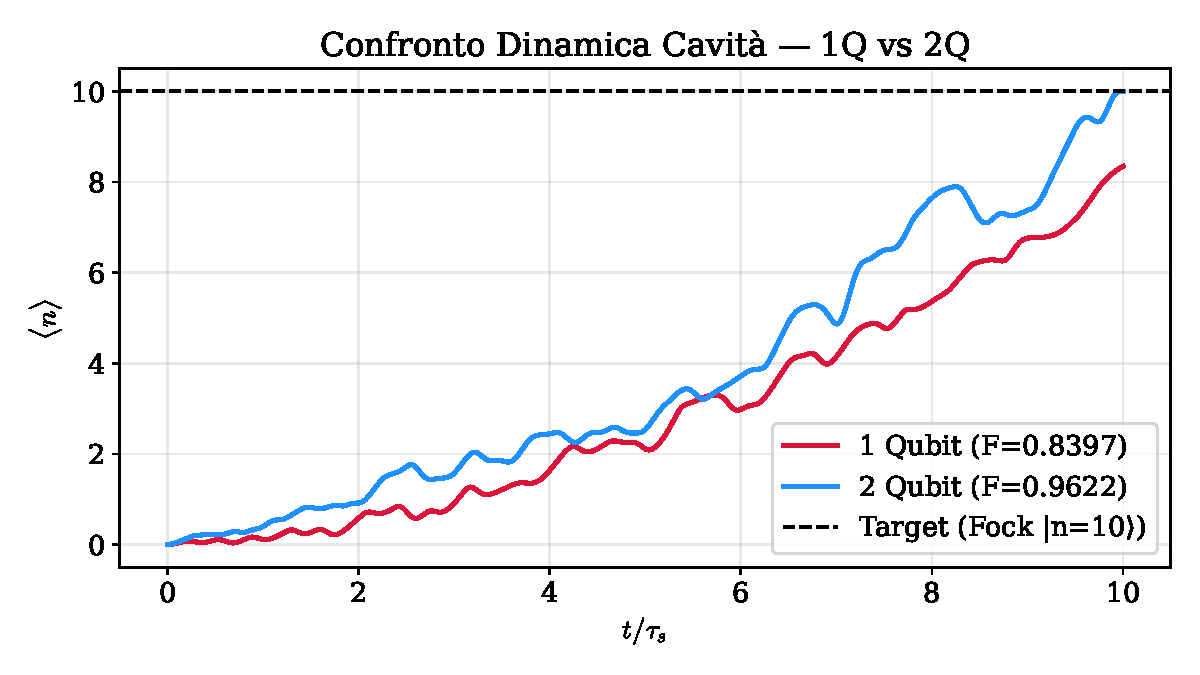
\includegraphics[width=\textwidth]{figure/v1_fock10_t10_comparison_nmean.pdf}
        \caption{Numero medio di fotoni $\langle n \rangle(t)$: 1Q vs 2Q}
    \end{subfigure}
    \hfill
    \begin{subfigure}[b]{0.48\textwidth}
        \centering
        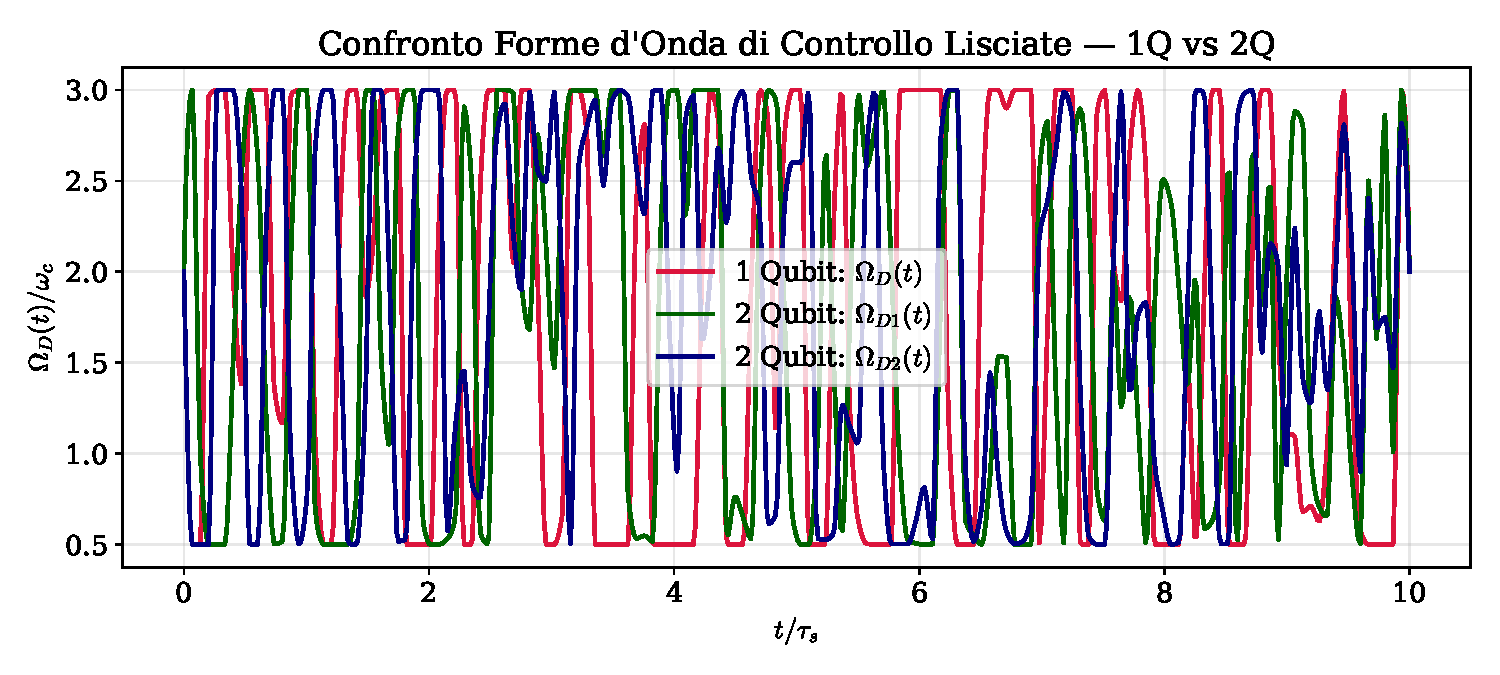
\includegraphics[width=\textwidth]{figure/v1_fock10_t10_comparison_drives.pdf}
        \caption{Controlli ottimali $\Omega_D(t)$ dopo PCHIP: 1Q vs 2Q}
    \end{subfigure}
\end{figure}

\begin{figure}[H]
    \centering
    \begin{subfigure}[b]{0.48\textwidth}
        \centering
        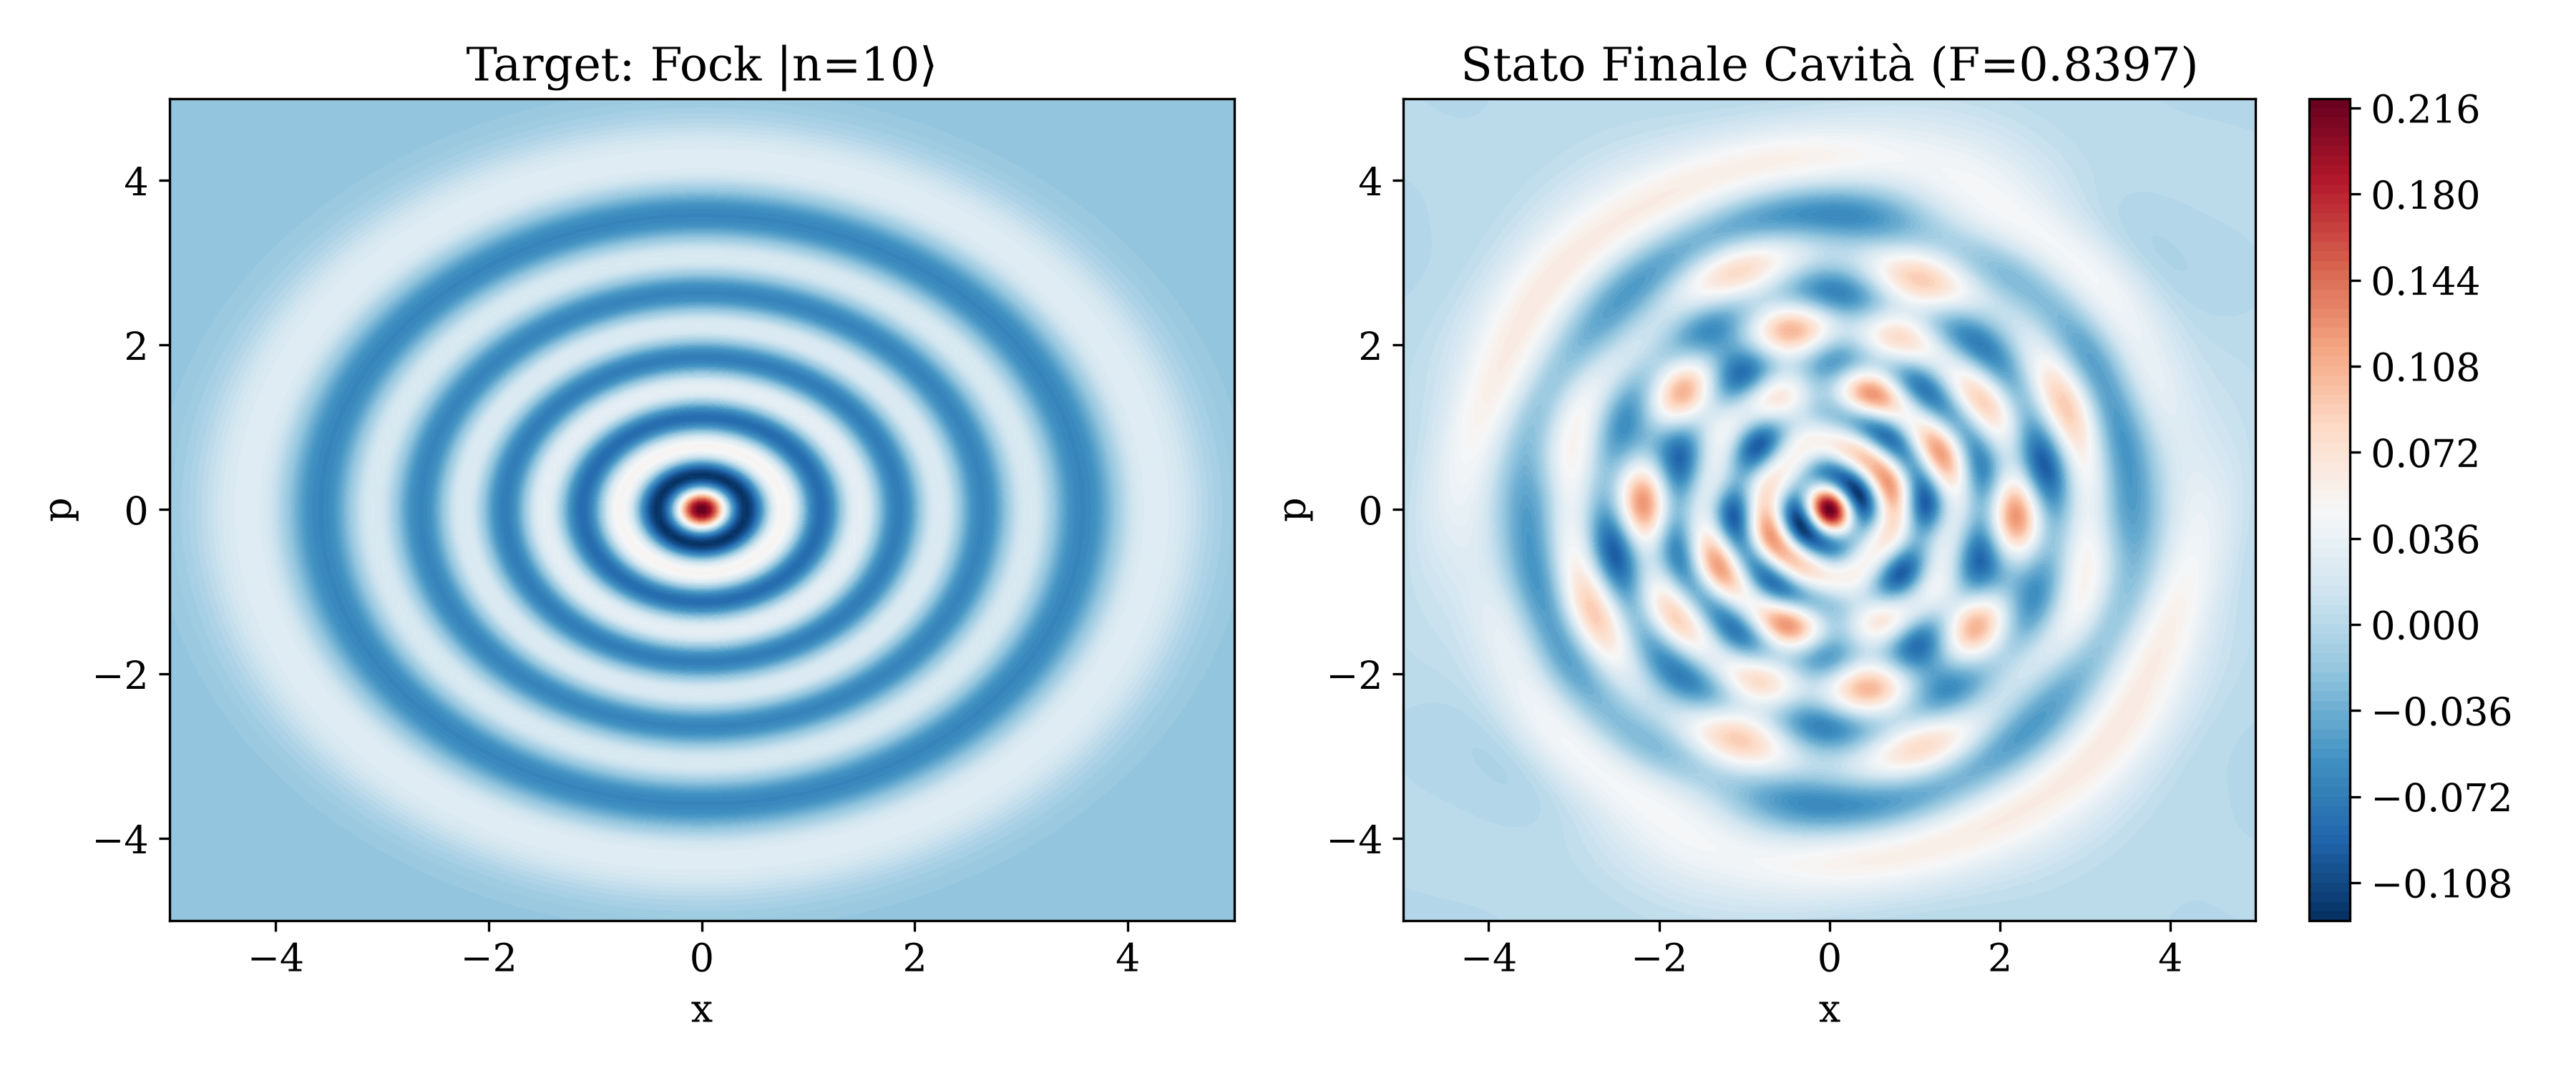
\includegraphics[width=\textwidth]{figure/v1_fock10_t10_1q_wigner.png}
        \caption{1Q ($T=10\,\tau_s$): $F_{\text{smooth}} = 0.8397$ (GRAPE $0.8720$)}
    \end{subfigure}
    \hfill
    \begin{subfigure}[b]{0.48\textwidth}
        \centering
        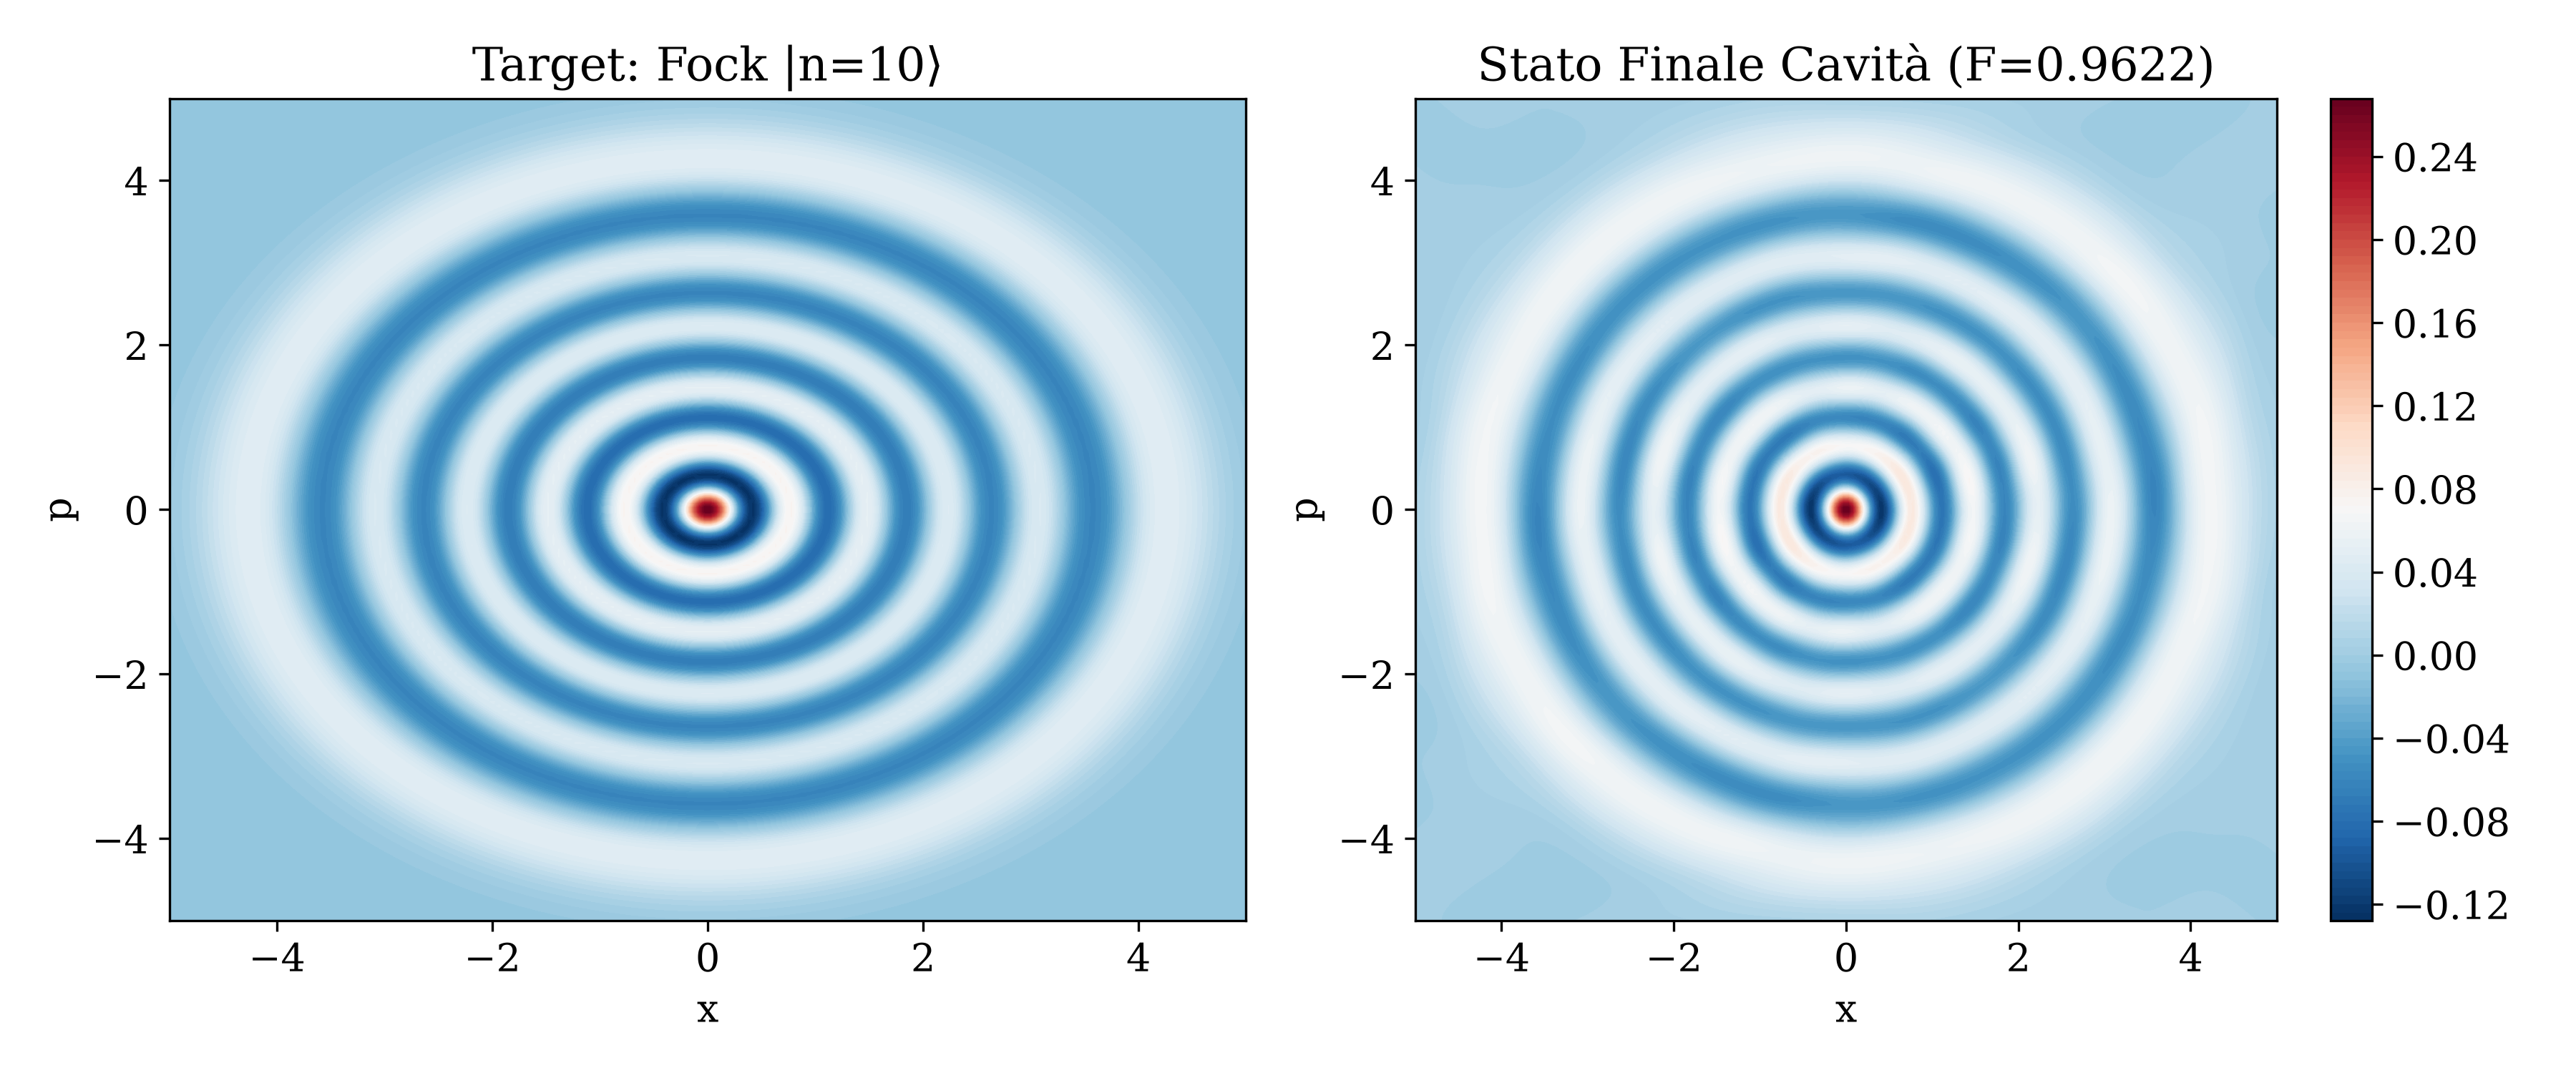
\includegraphics[width=\textwidth]{figure/v1_fock10_t10_2q_wigner.png}
        \caption{2Q ($T=10\,\tau_s$): $F_{\text{smooth}} = 0.9622$ (GRAPE $0.9988$)}
    \end{subfigure}
\end{figure}

\paragraph{2. Confronto 1Q vs 2Q sullo stato Cat a 4 componenti ($\alpha = 2.0$, $T=15\,\tau_s$):}
Nella run \texttt{run\_2026-10-03\_15-06-31} ho confrontato 1Q e 2Q sulla preparazione della sovrapposizione di stati gatto su assi ortogonali $|\psi_{\text{cat}}\rangle \propto |C_\alpha^+\rangle - |C_{i\alpha}^+\rangle$ con $\alpha = 2.0$ ($\langle n \rangle \approx 3.80$) a $T = 15\,\tau_s \approx 78.54\,\omega_c^{-1}$ (8 seed CRAB, 150 slot GRAPE).
Qui nella fase GRAPE entrambi i sistemi raggiungevano una fedeltà sopra $0.999$ ($0.99935$ per 1Q in 76 iterazioni e $0.99956$ per 2Q in 150 iterazioni), con slew rate più bassi sui due canali di 2Q ($\text{SR}_{\max} = 5.12$ e $6.24$ contro $6.33$ di 1Q). Tuttavia, appena applicata l'interpolazione PCHIP finale per rendere continuo il controllo a gradini, entrambi i sistemi crollavano di circa il 10\%, scendendo a $0.8945$ (1Q) e $0.8989$ (2Q). Con 150 slot su $T \approx 78.54$, il passo di GRAPE era largo ($\Delta t \approx 0.52\,\omega_c^{-1}$) e la struttura di interferenza a scacchiera dello stato Cat nello spazio delle fasi veniva compromessa dal cambio di forma d'onda tra gradini e spline cubica.

\begin{figure}[H]
    \centering
    \begin{subfigure}[b]{0.48\textwidth}
        \centering
        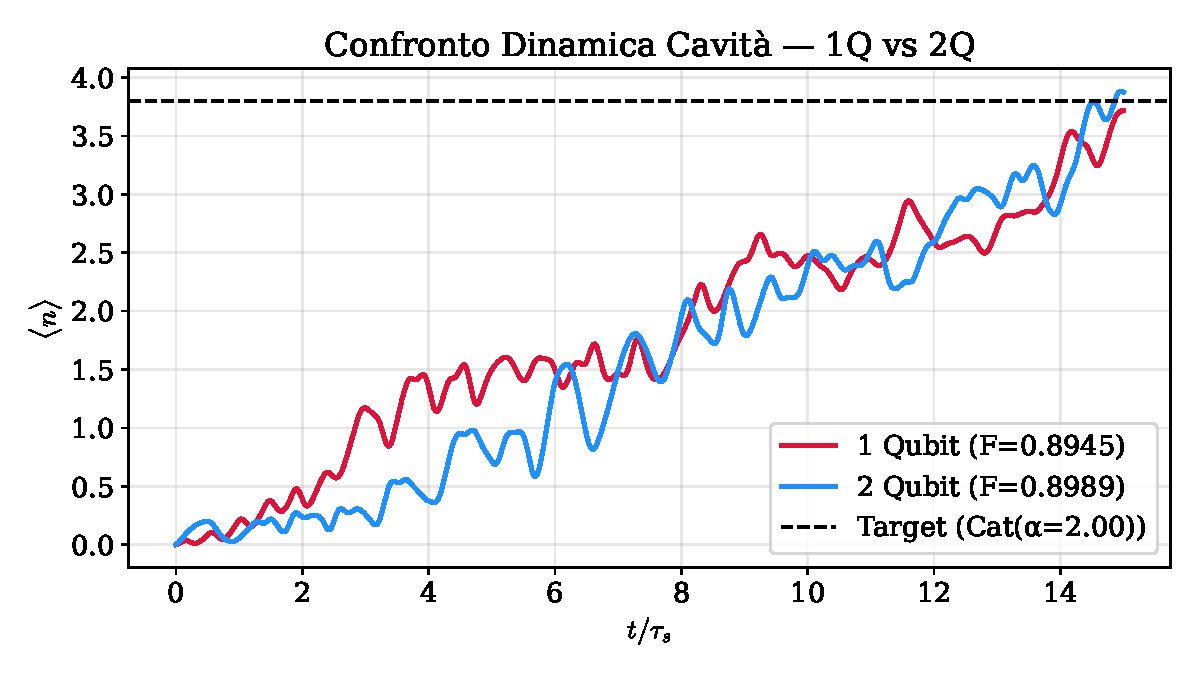
\includegraphics[width=\textwidth]{figure/v1_cat2_t15_comparison_nmean.pdf}
        \caption{Cat $\alpha=2.0$, $T=15\,\tau_s$: evoluzione di $\langle n \rangle(t)$}
    \end{subfigure}
    \hfill
    \begin{subfigure}[b]{0.48\textwidth}
        \centering
        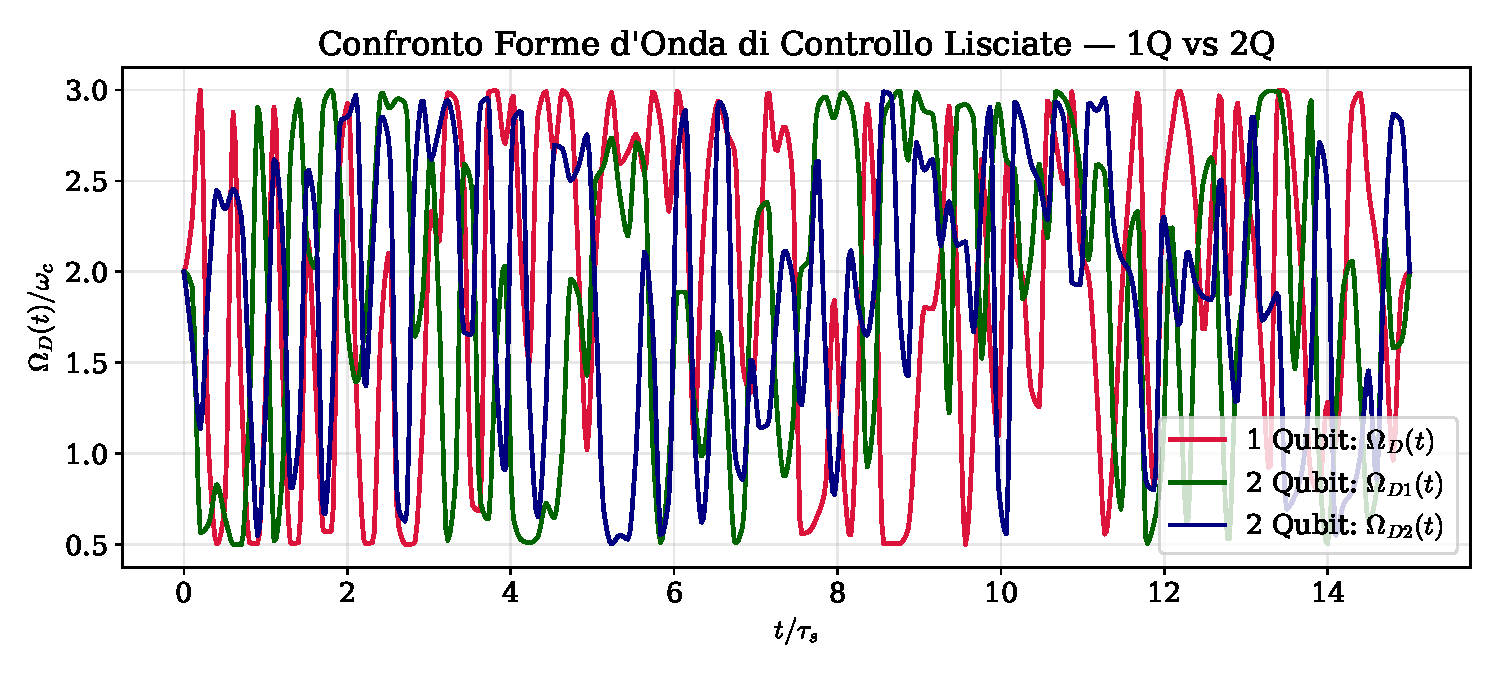
\includegraphics[width=\textwidth]{figure/v1_cat2_t15_comparison_drives.pdf}
        \caption{Cat $\alpha=2.0$, $T=15\,\tau_s$: controlli $\Omega_D(t)$ dopo PCHIP}
    \end{subfigure}
\end{figure}

\begin{figure}[H]
    \centering
    \begin{subfigure}[b]{0.48\textwidth}
        \centering
        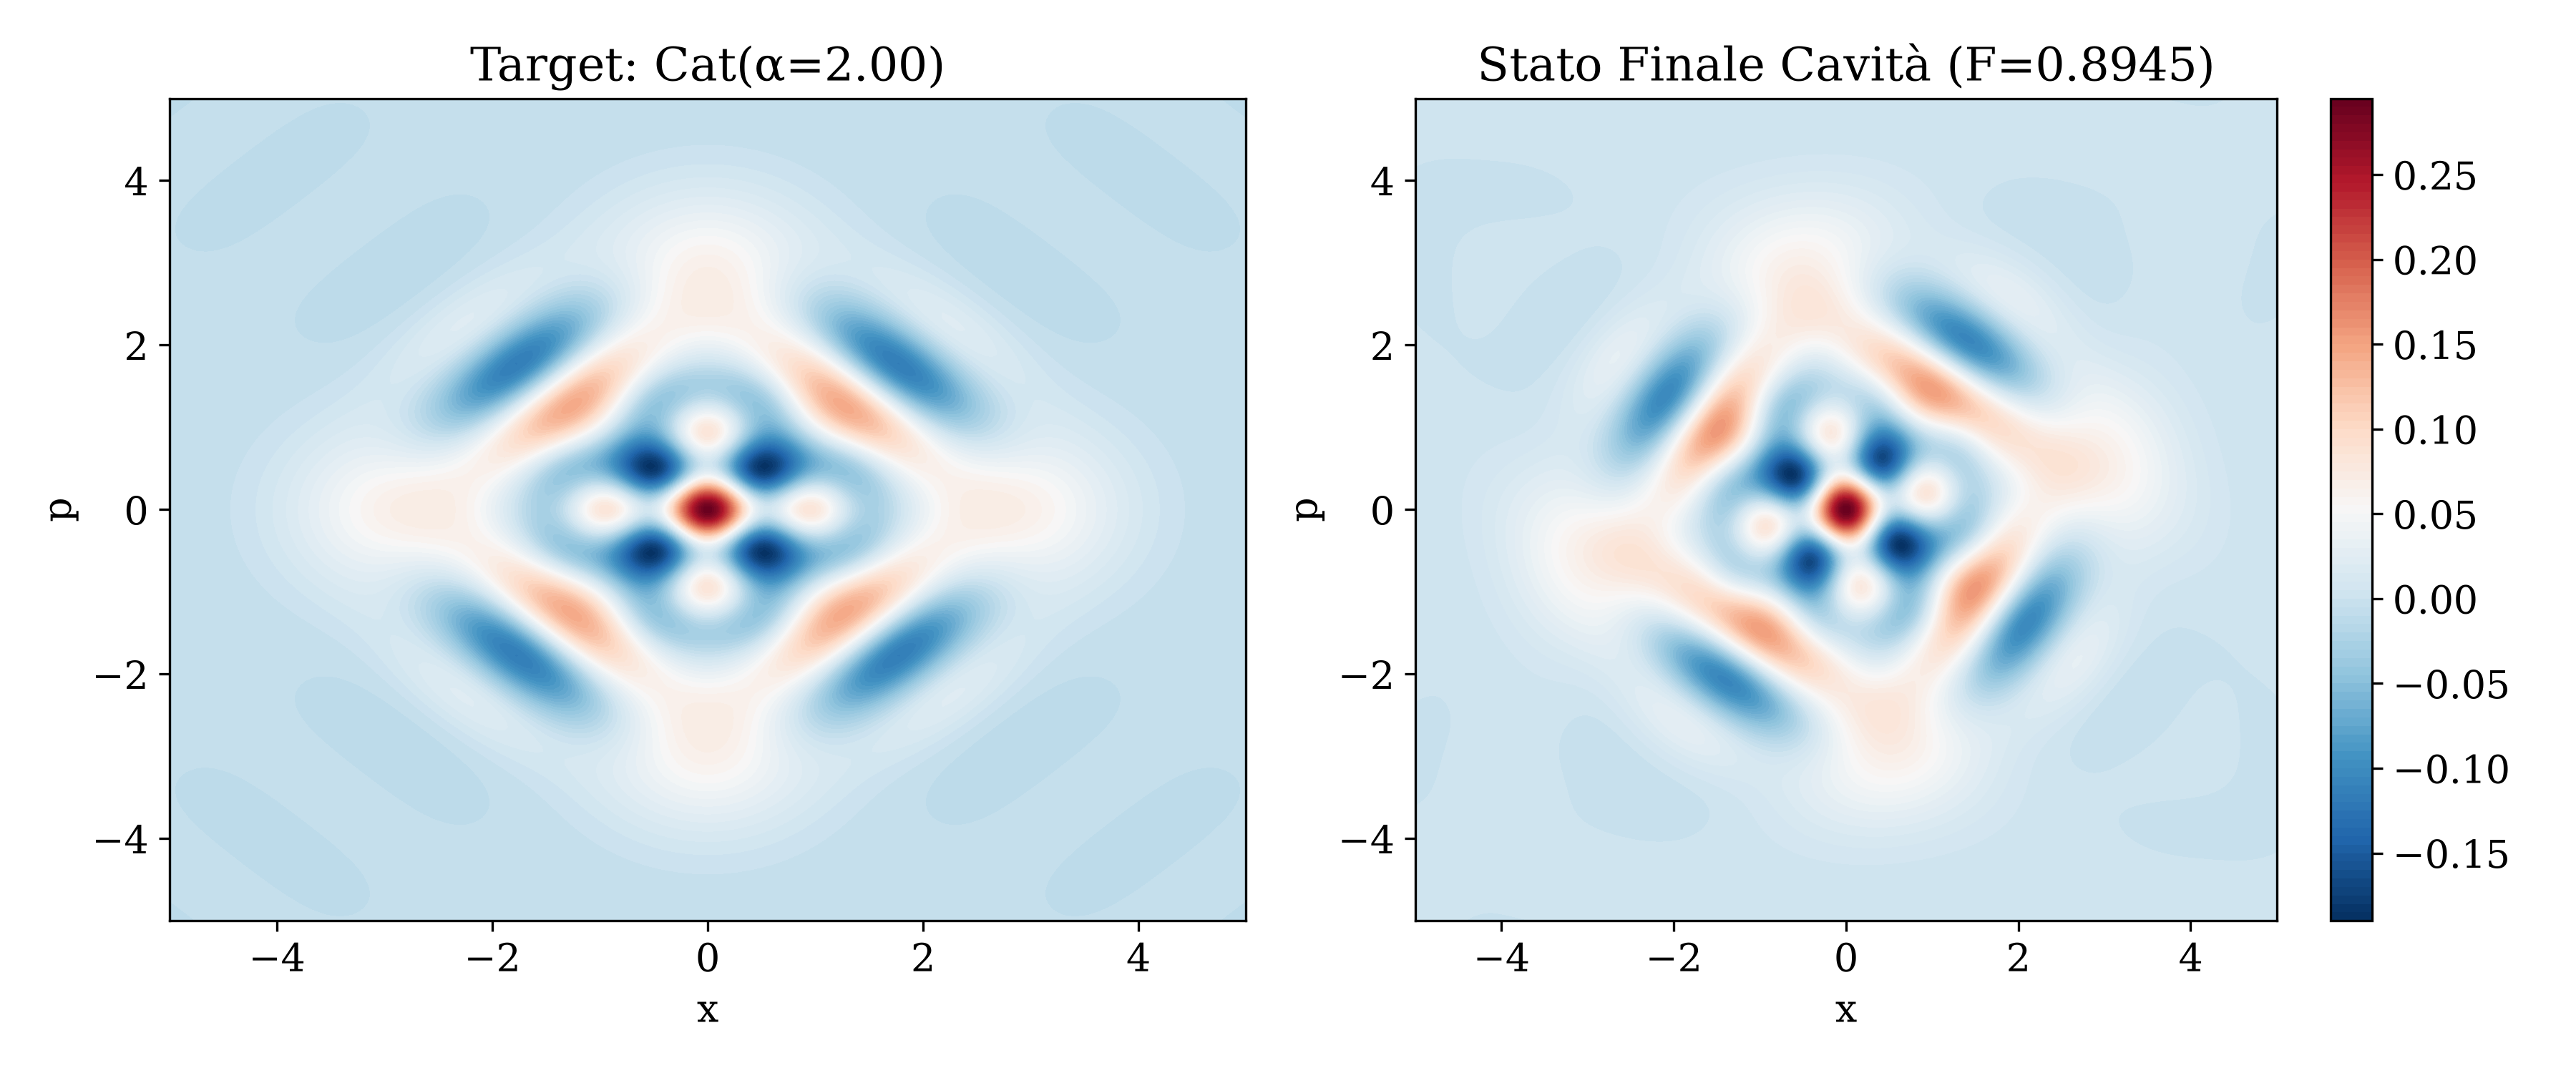
\includegraphics[width=\textwidth]{figure/v1_cat2_t15_1q_wigner.png}
        \caption{1Q ($T=15\,\tau_s$): GRAPE $0.9994 \to$ PCHIP $0.8945$}
    \end{subfigure}
    \hfill
    \begin{subfigure}[b]{0.48\textwidth}
        \centering
        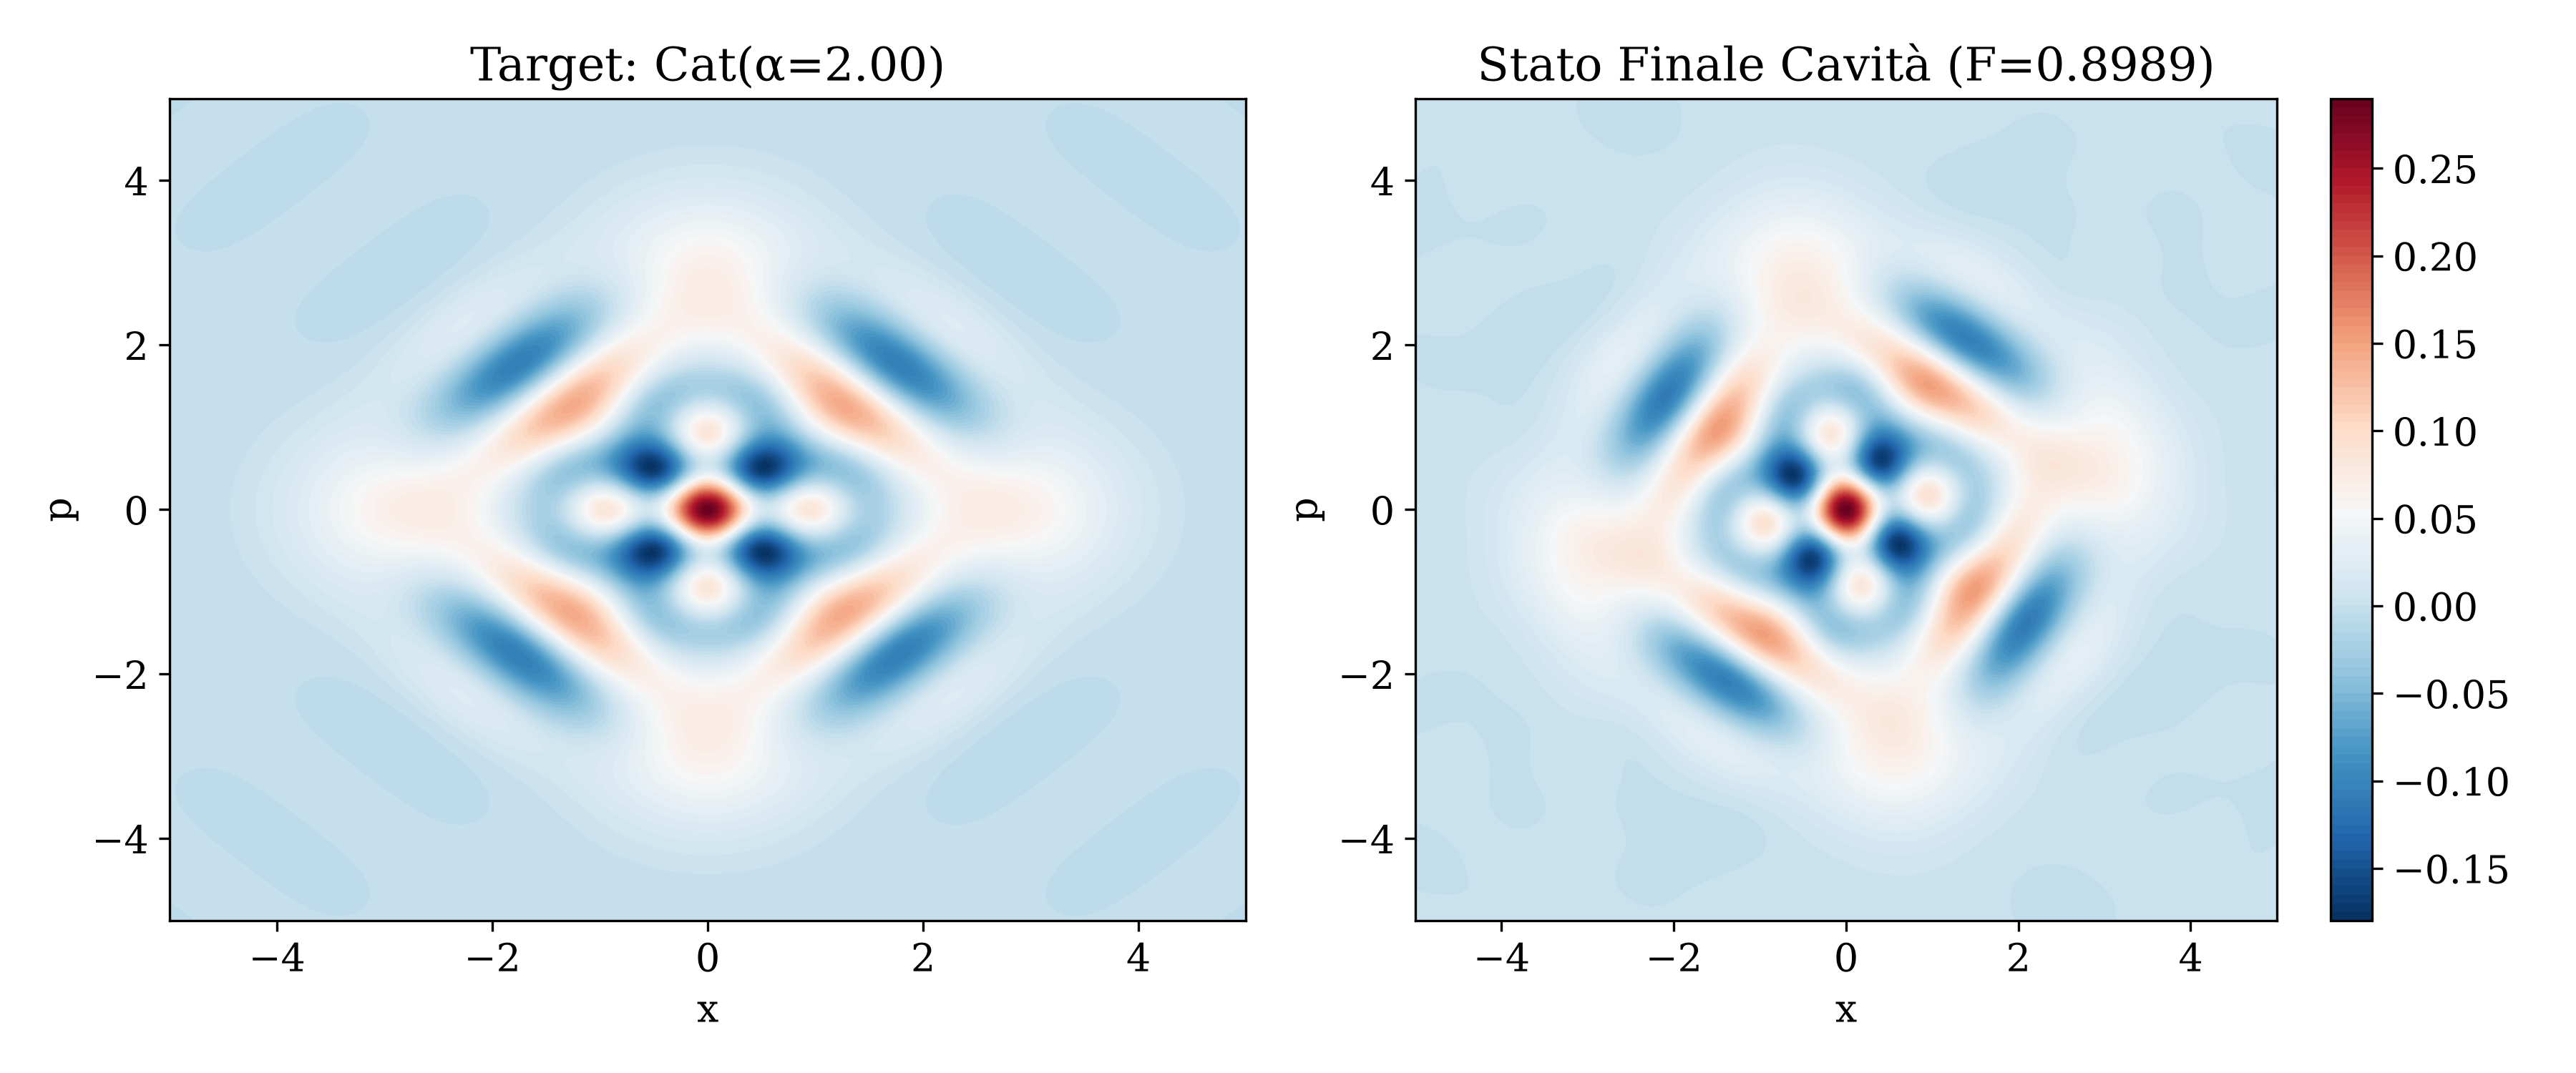
\includegraphics[width=\textwidth]{figure/v1_cat2_t15_2q_wigner.png}
        \caption{2Q ($T=15\,\tau_s$): GRAPE $0.9996 \to$ PCHIP $0.8989$}
    \end{subfigure}
\end{figure}

\subsection{I problemi emersi guardando i risultati della v1}
Analizzando questi numeri ho voluto provare a risolvere diverse problematiche:
\begin{itemize}
    \item \textbf{Il crollo dopo lo smoothing PCHIP:} ottimizzare un controllo a gradini in GRAPE e lisciarlo solo alla fine cambiava il segnale quel tanto che bastava per far perdere dal 2\% fino al 10\% di fedeltà (come nel caso Cat). In più, anche la verifica del segnale PCHIP veniva fatta ripassandolo al propagatore a gradini su $2 N_t$ punti, e non integrando l'equazione di Schrödinger continua.
    \item \textbf{GRAPE che peggiorava il risultato CRAB (caso 1Q a $T=10\,\tau_s$):} in v1 CRAB integrava con \texttt{sesolve} su 400 punti, mentre GRAPE ricampionava l'impulso su 150 slot costanti a tratti. Inoltre, creando la griglia con \texttt{np.linspace(0, T, Nt)} e applicando $N_t$ passi di durata $dt = T/(N_t - 1)$, l'evoluzione in GRAPE durava in realtà $N_t \cdot T/(N_t-1) > T$. A questo si aggiungeva il fatto che il gradiente era calcolato al primo ordine in $dt$ (usando il commutatore $[H_k, \rho_t]$), un'approssimazione che può risultare imprecisa quando gli slot temporali sono larghi.
    \item \textbf{Ambiguità nelle metriche:} in CRAB e dopo PCHIP veniva usata \texttt{qutip.fidelity}, che restituisce la radice dell'overlap $F_{\text{root}} = \sqrt{P_{\text{target}}}$, mentre GRAPE massimizzava direttamente la probabilità $P_{\text{target}} = \operatorname{Tr}[O_{\text{target}}\rho]$. Anche il costo $C^2$ integrava la frequenza totale $\Omega_j(t)^2$ (includendo quindi l'offset costante $\omega_q = 2$) invece della sola modulazione.
    \item \textbf{Mancanza di controlli sul troncamento di Fock:} con $n=10$ e $\text{dim}=40$, non avevo una verifica automatica che durante la dinamica la popolazione non andasse a sbattere sul bordo dello spazio troncato.
\end{itemize}

\newpage
\section{Cosa ho cambiato nella v2 e perché}

Per risolvere questi punti ho riscritto la pipeline da zero nella cartella autonoma \texttt{v2/} (lasciando intatti tutti i file e i risultati della v1) e l'ho controllata con una suite di 46 test automatici (gradienti contro differenze finite, limiti fisici a $g=0$, conservazione di norma e parità).

\begin{table}[H]
\centering
\small
\renewcommand{\arraystretch}{1.25}
\begin{tabular}{>{\raggedright\arraybackslash}p{2.6cm} >{\raggedright\arraybackslash}p{3.9cm} >{\raggedright\arraybackslash}p{4.3cm} >{\raggedright\arraybackslash}p{3.5cm}}
\toprule
\textbf{Aspetto} & \textbf{Come funzionava in v1} & \textbf{Come funziona in v2} & \textbf{Motivazione} \\
\midrule
\textbf{Forma del controllo e filtro} & Costante a tratti in GRAPE + smoothing PCHIP applicato solo a fine corsa. & Comando lineare a tratti su $M$ nodi (con estremi $\delta(0)=\delta(T)=0$) passato in un filtro causale del 1° ordine ($\omega_{\text{cut}} = 3.0$) calcolato analiticamente. & L'ottimizzatore modifica direttamente il segnale continuo filtrato. Sparisce la perdita da smoothing a posteriori. \\
\addlinespace
\textbf{Griglia temporale e propagazione} & Matrici densità complete; $N_t$ passi di ampiezza $T/(N_t-1)$. & Ket ridotti al settore di parità iniziale (dimensione dimezzata); $N$ intervalli midpoint di passo esatto $dt = T/N$. & L'evoluzione termina esattamente a $T$ ed è molto più veloce in memoria e calcolo. \\
\addlinespace
\textbf{Gradiente GRAPE} & Approssimazione al primo ordine nel passo $dt$ tramite commutatore. & Derivata esatta (Fréchet) dell'esponenziale di matrice nella base degli autovettori di ciascun passo. & \texttt{L-BFGS-B} riceve il gradiente esatto del costo discretizzato e conserva sempre il miglior punto visitato. \\
\addlinespace
\textbf{Validazione numerica} & Assente (solo rivalutazione a gradini su $2 N_t$ punti). & Propagazione continua indipendente (\texttt{sesolve}) confrontata con midpoint a $N$ e $2N$ passi (\texttt{time\_grid}), tolleranze ODE ridotte di $10\times$ e dimensione aumentata di $+20$ livelli (\texttt{dimension}, distanza di traccia e popolazione di bordo). & Un risultato viene accettato (\texttt{Validato = True}) solo se il segnale continuo riproduce la fedeltà discreta e non risente del troncamento di Fock. \\
\addlinespace
\textbf{Definizione di fedeltà} & Mista tra $P_{\text{target}}$ e $\sqrt{P_{\text{target}}}$. & Salvataggio separato di $P_{\text{target}}$ e $F_{\text{root}} = \sqrt{P_{\text{target}}}$. Soglia di successo ($0.99$) posta su $P_{\text{target}}$. & Evita ambiguità tra probabilità e radice della probabilità. \\
\addlinespace
\textbf{Statistica sui seed e casi} & 1Q vs 2Q; solo il miglior seed CRAB veniva passato a GRAPE. & 5 casi fisici confrontati; tutti gli 8 seed vengono raffinati con GRAPE. & Valuta la frequenza di successo reale e separa accoppiamento collettivo e numero di canali. \\
\bottomrule
\end{tabular}
\label{tab:cambiamenti_v2}
\end{table}

\subsection*{Nota sul calcolo esatto del gradiente (derivata di Fréchet)}
Nel propagatore midpoint della v2, su ciascun intervallo temporale $k$ di ampiezza $dt = T/N$ l'Hamiltoniana è costante a tratti, $H_k = H_0 + \sum_j u_{j,k} H_{c,j}$, e il passo di evoluzione è $U_k = e^{-i\,dt\,H_k}$. Per calcolare il gradiente rispetto all'ampiezza di controllo $u_{j,k}$ serve la derivata dell'esponenziale di matrice $\partial U_k / \partial u_{j,k}$.

\noindent
Poiché l'operatore di controllo $H_{c,j}$ (proporzionale a $\sigma_z$) non commuta con l'Hamiltoniana totale $H_k$ (che contiene i termini di scambio fotonico $\sigma_x(a+a^\dagger)$), non vale la regola scalare $\frac{\partial}{\partial u}e^{-i\,dt\,H_k} = -i\,dt\,H_{c,j} U_k$. Nella v1 veniva usata proprio questa approssimazione al primo ordine in $dt$ (tramite il commutatore $[H_{c,j}, \rho_k]$), che però trascura tutti i termini di ordine $\mathcal{O}(dt^2)$ legati alla non-commutatività durante il passo $dt$ e introduce un errore sistematico nella direzione di discesa di \texttt{L-BFGS-B}.

\noindent
Nella v2 ho invece implementato la derivata di Fréchet esatta dell'esponenziale di matrice sfruttando la diagonalizzazione $H_k = V_k \operatorname{diag}(E_a) V_k^\dagger$ già calcolata per propagare lo stato. Nella base degli autovettori istantanei di $H_k$, gli elementi di matrice della derivata esatta hanno la forma chiusa (formula di Daleckii--Krein):
\begin{equation}
    \left(V_k^\dagger \frac{\partial U_k}{\partial u_{j,k}} V_k\right)_{ab} = \left(V_k^\dagger H_{c,j} V_k\right)_{ab} \cdot G_{ab}, \qquad
    G_{ab} = -i\,dt\,e^{-i\,dt\,(E_a + E_b)/2}\,\operatorname{sinc}\!\left(\frac{dt\,(E_a - E_b)}{2\pi}\right),
\end{equation}
dove $\operatorname{sinc}(x) = \sin(\pi x)/(\pi x)$ vale $1$ per $x=0$, rendendo l'espressione numericamente stabile anche in presenza di autovalori degeneri ($E_a = E_b$). In questo modo il gradiente delle ampiezze midpoint (poi riportato ai nodi del comando tramite la matrice analitica del filtro) coincide con la derivata esatta della funzione costo discretizzata fino alla precisione di macchina ($\sim 10^{-15}$). Questa formulazione spettrale per il gradiente esatto in GRAPE è descritta in dettaglio in:
\begin{itemize}
    \item S.~Machnes \emph{et al.}, \emph{``Comparing, Optimizing, and Benchmarking Quantum-Control Algorithms in a Unifying Programming Framework''}, Phys.\ Rev.\ A \textbf{84}, 022305 (2011) — disponibile su arXiv: \href{https://arxiv.org/abs/1011.4874}{\texttt{arXiv:1011.4874}} (Appendice~A / Sez.~II.B sulla derivata esatta dell'esponenziale tramite autodecomposizione);
    \item P.~de~Fouquieres, S.~G.~Schirmer, S.~J.~Glaser, I.~Kuprov, \emph{``Second order gradient ascent pulse engineering''}, J.\ Magn.\ Reson.\ \textbf{212}, 412--417 (2011) — disponibile su arXiv: \href{https://arxiv.org/abs/1102.4096}{\texttt{arXiv:1102.4096}} (mostra perché il gradiente approssimato al primo ordine blocca la convergenza di \texttt{L-BFGS-B} e ricava la derivata esatta del propagatore).
\end{itemize}

\noindent
(Articoli di riferimento, ho utilizzato gemini per capire se e come implementarli nel nostro caso).

\subsection*{Scelta della funzione obiettivo \texttt{root} e configurazione dei 5 casi}
Quando si cercano stati di Fock ad alto numero di fotoni (come $|n=10\rangle$) partendo dal vuoto $|0,g\rangle$, all'inizio della ricerca la probabilità di occupazione del target $P_{\text{target}}$ è prossima a zero ($\sim 10^{-8}$). Usando la funzione costo lineare nella probabilità $J_{\text{prob}} = 1 - P_{\text{target}}$, in quella regione il paesaggio è quasi piatto e il gradiente è così piccolo da far fermare subito \texttt{L-BFGS-B} per tolleranza sul gradiente. Per evitare questo blocco ho introdotto nella campagna v2 l'obiettivo radice regolarizzato (\texttt{root}):
\begin{equation}
    J_{\text{root}} = \sqrt{1 + \varepsilon} - \sqrt{P_{\text{target}} + \varepsilon} + \text{penalità}, \qquad \varepsilon = 10^{-12},
\end{equation}
il cui gradiente rispetto ai parametri di controllo è moltiplicato per il fattore:
\begin{equation}
    \frac{\partial J_{\text{root}}}{\partial u} = -\frac{1}{2\sqrt{P_{\text{target}} + \varepsilon}}\,\frac{\partial P_{\text{target}}}{\partial u}.
\end{equation}
Quando $P_{\text{target}} \ll 1$, il fattore $1/(2\sqrt{P_{\text{target}} + \varepsilon})$ amplifica automaticamente la derivata senza alterare la direzione del gradiente né la posizione degli ottimi (mentre le metriche salvate nei report restano sempre $P_{\text{target}}$ e $F_{\text{root}} = \sqrt{P_{\text{target}}}$ senza regolarizzazione). Inoltre ho alzato lo spazio di Fock a $\text{dim}=60$ (con verifica di convergenza a $\text{dim}=80$) e il budget a 6000 valutazioni CRAB e 600 iterazioni GRAPE.

\medskip
\noindent
Per rendere equo il confronto tra uno e due qubit, ogni esperimento in v2 mette a confronto 5 configurazioni:
\begin{enumerate}
    \item \texttt{1q}: un qubit con $g = 0.3$;
    \item \texttt{2q\_common}: due qubit con $g_1 = g_2 = 0.3$ pilotati dallo stesso segnale di modulazione (1 canale);
    \item \texttt{2q\_independent}: due qubit con $g_1 = g_2 = 0.3$ pilotati da due segnali indipendenti (2 canali);
    \item \texttt{2q\_normalized\_common}: due qubit con $g_1 = g_2 = 0.3/\sqrt{2} \approx 0.2121$ (così $\sqrt{g_1^2+g_2^2} = 0.3$ come in 1Q) e 1 canale comune;
    \item \texttt{2q\_normalized\_independent}: due qubit con $g_1 = g_2 = 0.3/\sqrt{2}$ e 2 canali indipendenti.
\end{enumerate}

\section{Risultati della campagna v2 (stato attuale)}

La campagna principale comprende 320 pipeline (8 seed $\times$ 5 sistemi $\times$ 8 esperimenti):
\begin{itemize}
    \item \textbf{Blocco filtrato ($\omega_{\text{cut}} = 3.0$):} stati di Fock $n = 2, 6, 10$ a due durate, $T = 10\,\tau_s$ ($1000$ intervalli, $101$ nodi) e $T = 20\,\tau_s$ ($2000$ intervalli, $201$ nodi).
    \item \textbf{Blocco diagnostico senza filtro ($\omega_{\text{cut}} = \text{null}$):} stato di Fock $n = 10$ a $T = 10\,\tau_s$ e $T = 20\,\tau_s$, per isolare quanto del limite a tempi brevi dipenda dal filtro passa-basso e quanto dalla dinamica del sistema.
\end{itemize}

Al momento sono terminati 7 esperimenti principali su 8 (\texttt{main\_004}--\texttt{main\_010}); manca solo \texttt{main\_011} (Fock 10 a $T = 20\,\tau_s$ senza filtro). I risultati completi dei blocchi filtrati sono riassunti nella Figura~\ref{fig:panoramica_campagna} e nella Tabella~\ref{tab:risultati_campagna}.

\begin{figure}[H]
    \centering
    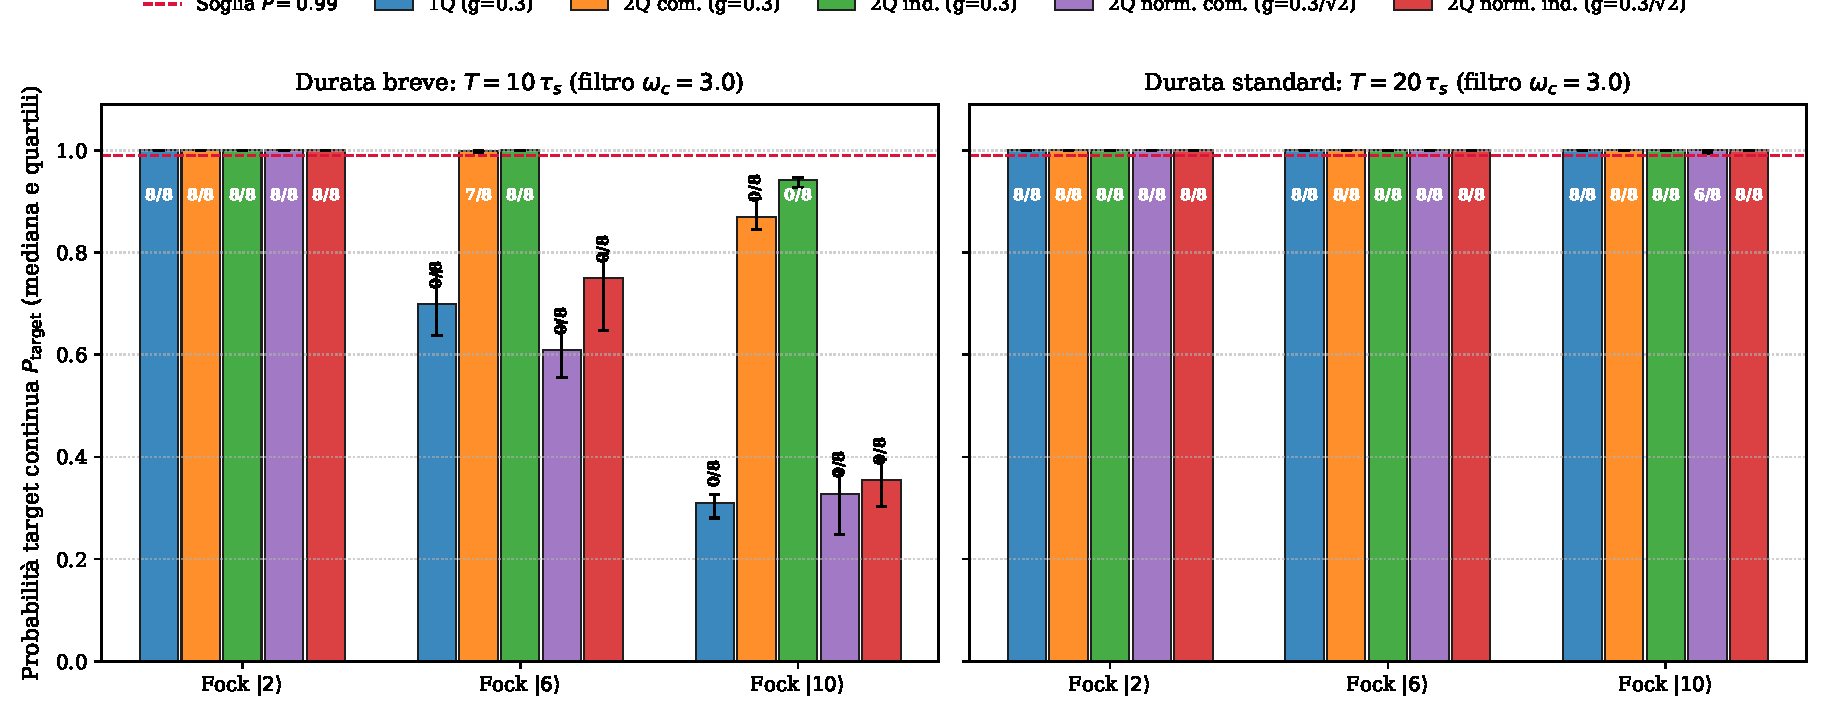
\includegraphics[width=\textwidth]{figure/fig1_panoramica_campagna.pdf}
    \caption{Panoramica dei 6 blocchi principali con filtro causale ($\omega_{\text{cut}}=3.0$): probabilità target continua $P_{\text{target}}$ (mediana e intervallo interquartile su 8 seed) a durata breve $T=10\,\tau_s$ (\texttt{main\_004}, \texttt{main\_006}, \texttt{main\_008}, a sinistra) e a durata standard $T=20\,\tau_s$ (\texttt{main\_005}, \texttt{main\_007}, \texttt{main\_009}, a destra). Sopra o dentro ogni barra è indicato il numero di seed (su 8) che superano sia la soglia $P \ge 0.99$ sia tutti i controlli di validazione numerica.}
    \label{fig:panoramica_campagna}
\end{figure}

\begin{table}[H]
\centering
\footnotesize
\setlength{\tabcolsep}{4pt}
\renewcommand{\arraystretch}{1.15}
\resizebox{\textwidth}{!}{%
\begin{tabular}{llcccl}
\toprule
\textbf{Esperimento} & \textbf{Sistema} & \textbf{Successi validati} & \textbf{$P_{\text{target}}$ mediana} & \textbf{$P_{\text{target}}$ $[\min, \max]$} & \textbf{Esito validazione numerica} \\
\midrule
\multirow{5}{*}{\shortstack[l]{\textbf{Fock $n=2$, $T=10\,\tau_s$}\\filtro $3.0$ (\texttt{main\_004})}}
 & \texttt{1q} & \textbf{8/8} & 0.999997 & $[0.999996, 0.999998]$ & 8/8 validati \\
 & \texttt{2q\_common} & \textbf{8/8} & 0.999996 & $[0.999993, 0.999998]$ & 8/8 validati \\
 & \texttt{2q\_independent} & \textbf{8/8} & 0.999997 & $[0.999996, 0.999998]$ & 8/8 validati \\
 & \texttt{2q\_norm\_common} & \textbf{8/8} & 0.999990 & $[0.999693, 0.999996]$ & 8/8 validati \\
 & \texttt{2q\_norm\_independent} & \textbf{8/8} & 0.999994 & $[0.999991, 0.999996]$ & 8/8 validati \\
\midrule
\textbf{Fock $n=2$, $T=20\,\tau_s$} (\texttt{main\_005}) & Tutti i 5 sistemi & \textbf{8/8} & $\ge 0.999997$ & $[\ge 0.999995, 0.999999]$ & 8/8 validati in ogni caso \\
\midrule
\multirow{5}{*}{\shortstack[l]{\textbf{Fock $n=6$, $T=10\,\tau_s$}\\filtro $3.0$ (\texttt{main\_006})}}
 & \texttt{1q} & \textbf{0/8} & 0.698929 & $[0.596857, 0.776816]$ & 0/8 (fallisce \texttt{time\_grid}) \\
 & \texttt{2q\_common} & \textbf{7/8} & 0.998268 & $[0.986730, 0.999982]$ & 8/8 validati (1 seed a 0.987) \\
 & \texttt{2q\_independent} & \textbf{8/8} & 0.999987 & $[0.999963, 0.999994]$ & 8/8 validati \\
 & \texttt{2q\_norm\_common} & \textbf{0/8} & 0.609237 & $[0.393262, 0.750650]$ & 0/8 (fallisce \texttt{time\_grid}) \\
 & \texttt{2q\_norm\_independent} & \textbf{0/8} & 0.749373 & $[0.577314, 0.837847]$ & 0/8 (fallisce \texttt{time\_grid}) \\
\midrule
\multirow{5}{*}{\shortstack[l]{\textbf{Fock $n=6$, $T=20\,\tau_s$}\\filtro $3.0$ (\texttt{main\_007})}}
 & \texttt{1q} & \textbf{8/8} & 0.999996 & $[0.999996, 0.999997]$ & 8/8 validati \\
 & \texttt{2q\_common} & \textbf{8/8} & 0.999997 & $[0.999996, 0.999998]$ & 8/8 validati \\
 & \texttt{2q\_independent} & \textbf{8/8} & 0.999996 & $[0.999993, 0.999998]$ & 8/8 validati \\
 & \texttt{2q\_norm\_common} & \textbf{8/8} & 0.999989 & $[0.999982, 0.999992]$ & 8/8 validati \\
 & \texttt{2q\_norm\_independent} & \textbf{8/8} & 0.999993 & $[0.999989, 0.999994]$ & 8/8 validati \\
\midrule
\multirow{5}{*}{\shortstack[l]{\textbf{Fock $n=10$, $T=10\,\tau_s$}\\filtro $3.0$ (\texttt{main\_008})}}
 & \texttt{1q} & \textbf{0/8} & 0.310186 & $[0.271406, 0.352806]$ & 0/8 (fallisce \texttt{time\_grid}) \\
 & \texttt{2q\_common} & \textbf{0/8} & 0.869445 & $[0.802777, 0.936308]$ & 0/8 (fallisce \texttt{time\_grid}) \\
 & \texttt{2q\_independent} & \textbf{0/8} & 0.940965 & $[0.875524, 0.961781]$ & 0/8 (fallisce \texttt{time\_grid}) \\
 & \texttt{2q\_norm\_common} & \textbf{0/8} & 0.328171 & $[0.179080, 0.442175]$ & 0/8 (fallisce \texttt{time\_grid}) \\
 & \texttt{2q\_norm\_independent} & \textbf{0/8} & 0.355114 & $[0.294268, 0.467935]$ & 0/8 (fallisce \texttt{time\_grid}) \\
\midrule
\multirow{5}{*}{\shortstack[l]{\textbf{Fock $n=10$, $T=20\,\tau_s$}\\filtro $3.0$ (\texttt{main\_009})}}
 & \texttt{1q} & \textbf{8/8} & 0.999992 & $[0.999982, 0.999995]$ & 8/8 validati \\
 & \texttt{2q\_common} & \textbf{8/8} & 0.999996 & $[0.999994, 0.999997]$ & 8/8 validati \\
 & \texttt{2q\_independent} & \textbf{8/8} & 0.999994 & $[0.999990, 0.999995]$ & 8/8 validati \\
 & \texttt{2q\_norm\_common} & \textbf{6/8} & 0.999956 & $[0.972811, 0.999985]$ & 6/8 validati (2 falliscono \texttt{time\_grid}) \\
 & \texttt{2q\_norm\_independent} & \textbf{8/8} & 0.999986 & $[0.999984, 0.999993]$ & 8/8 validati \\
\midrule
\multirow{5}{*}{\shortstack[l]{\textbf{Fock $n=10$, $T=10\,\tau_s$}\\senza filtro (\texttt{main\_010})}}
 & \texttt{1q} & \textbf{0/8} & 0.635531 & $[0.573466, 0.703158]$ & 0/8 (fallisce \texttt{time\_grid}) \\
 & \texttt{2q\_common} & \textbf{2/8} & 0.981896 & $[0.967130, 0.999879]$ & 2/8 validati (6 falliscono \texttt{time\_grid}) \\
 & \texttt{2q\_independent} & \textbf{8/8} & 0.999937 & $[0.999414, 0.999970]$ & 8/8 validati \\
 & \texttt{2q\_norm\_common} & \textbf{0/8} & 0.561297 & $[0.506857, 0.676184]$ & 0/8 (fallisce \texttt{time\_grid}) \\
 & \texttt{2q\_norm\_independent} & \textbf{0/8} & 0.730965 & $[0.598527, 0.829199]$ & 0/8 (fallisce \texttt{time\_grid}) \\
\midrule
\textbf{Fock $n=10$, $T=20\,\tau_s$} (\texttt{main\_011}) & Tutti i 5 sistemi & \emph{[In corso]} & \emph{[In corso]} & \emph{[In corso]} & \todo{inserire esiti \texttt{main\_011}} \\
\bottomrule
\end{tabular}%
}
\caption{Risultati della campagna v2 sui blocchi completati (\texttt{main\_004}--\texttt{main\_010}).}
\label{tab:risultati_campagna}
\end{table}

\subsection*{Cosa indicano questi dati sul confronto 1Q vs 2Q}

\begin{enumerate}
    \item \textbf{A tempi lunghi ($T = 20\,\tau_s$) tutti i sistemi preparano lo stato, anche 1Q e i casi normalizzati:}
    Sia per $n=2$, sia per $n=6$, sia per $n=10$, a $T=20\,\tau_s$ con filtro attivo il singolo qubit (\texttt{1q}) e i due qubit con accoppiamento normalizzato (\texttt{2q\_normalized\_independent}) centrano l'obiettivo su \textbf{8/8 seed}, con probabilità certificate superiori a $0.99998$ (Figura~\ref{fig:wigner_main009}). Soltanto \texttt{2q\_normalized\_common} su $n=10$ fallisce su 2 seed su 8 (fermandosi comunque a $P \approx 0.973 - 0.975$). Quindi, quando il tempo di interazione è $20\,\tau_s$, un singolo qubit è perfettamente in grado di generare anche Fock $|n=10\rangle$ con il filtro attivo.

    \item \textbf{A tempi brevi ($T = 10\,\tau_s$) emerge un vantaggio netto dei 2 qubit, ma legato soprattutto all'accoppiamento collettivo $\sqrt{2}g$:}
    Guardando \texttt{main\_006} (Fock $n=6$ a $T=10\,\tau_s$, Figura~\ref{fig:dinamica_fock6_t10}), i due sistemi con accoppiamento pieno per singolo qubit ($g_1=g_2=0.3$) raggiungono la soglia in modo certificato (\texttt{2q\_independent} con \textbf{8/8} seed e mediana $0.999987$; \texttt{2q\_common} con \textbf{7/8} seed e mediana $0.998268$). Al contrario, \texttt{1q} si ferma a una mediana di $0.6989$ (0/8), e i due sistemi a due qubit con accoppiamento riscalato $g_j = 0.3/\sqrt{2}$ (\texttt{2q\_normalized\_common} a $0.6092$ e \texttt{2q\_normalized\_independent} a $0.7494$) restano anch'essi a 0/8 su valori molto vicini a \texttt{1q}.
    Lo stesso schema si ripete su Fock $n=10$ a $T=10\,\tau_s$ (\texttt{main\_008} e \texttt{main\_010}): i casi \texttt{2q\_normalized} hanno sempre prestazioni paragonabili a \texttt{1q} e molto lontane da quelle di \texttt{2q\_common} e \texttt{2q\_independent}. Questo mostra chiaramente che la possibilità di dimezzare il tempo di preparazione da $20\,\tau_s$ a $10\,\tau_s$ per stati ad alto numero di fotoni dipende prima di tutto dall'aumento dell'accoppiamento efficace ($\sqrt{g_1^2+g_2^2} = \sqrt{2}g$).

    \item \textbf{Il ruolo del secondo canale indipendente (\texttt{2q\_independent} vs \texttt{2q\_common}):}
    A parità di accoppiamento fisico ($g_1=g_2=0.3$), avere due controlli indipendenti invece di un controllo comune dà un vantaggio visibile quando il problema diventa più stretto:
    \begin{itemize}
        \item su Fock $n=6$ a $T=10\,\tau_s$ (\texttt{main\_006}), \texttt{2q\_independent} porta a termine 8/8 seed con mediana $0.999987$ contro i 7/8 di \texttt{2q\_common} (mediana $0.998268$);
        \item su Fock $n=10$ a $T=10\,\tau_s$ senza filtro (\texttt{main\_010}, Figura~\ref{fig:filtro_vs_nofiltro}), \texttt{2q\_independent} valida \textbf{8/8} seed sopra soglia (mediana $0.999937$), mentre \texttt{2q\_common} si ferma a \textbf{2/8} seed validati (mediana $0.981896$).
    \end{itemize}
    Anche a parità di accoppiamento normalizzato ($g_j = 0.3/\sqrt{2}$), \texttt{2q\_normalized\_independent} ottiene sistematicamente mediane più alte di \texttt{2q\_normalized\_common} nei regimi non conversi a $10\,\tau_s$ ($0.749$ vs $0.609$ su $n=6$; $0.731$ vs $0.561$ su $n=10$ senza filtro) e 8/8 contro 6/8 su $n=10$ a $20\,\tau_s$. Tuttavia, da solo (senza l'aumento di $g_{\text{eff}}$), il secondo canale non basta a far raggiungere la soglia $0.99$ a $T=10\,\tau_s$ per $n=6$ o $n=10$.

    \item \textbf{L'effetto del filtro passa-basso a $T = 10\,\tau_s$ su Fock $n=10$ (\texttt{main\_008} vs \texttt{main\_010}):}
    Confrontando \texttt{main\_008} (con filtro $\omega_{\text{cut}}=3.0$) e \texttt{main\_010} (senza filtro) in Figura~\ref{fig:filtro_vs_nofiltro}, si vede perché a $T=10\,\tau_s$ con filtro nemmeno \texttt{2q\_independent} superava $0.99$ (fermandosi a mediana $0.9410$, max $0.9618$): il filtro con polo a $3\omega_c$ attenua le variazioni rapide sui 101 nodi di comando. Togliendo il filtro (\texttt{main\_010}), \texttt{2q\_independent} sale subito a \textbf{8/8} successi validati ($P_{\text{mediana}} = 0.999937$), usando una banda $\omega_{99\%} \approx 7.6 - 8.4\,\omega_c$. Invece \texttt{1q} e \texttt{2q\_normalized}, anche togliendo il filtro, salgono da $\sim 0.31 - 0.35$ a $\sim 0.56 - 0.73$ ma restano lontani dalla soglia $0.99$.
\end{enumerate}

\begin{figure}[H]
    \centering
    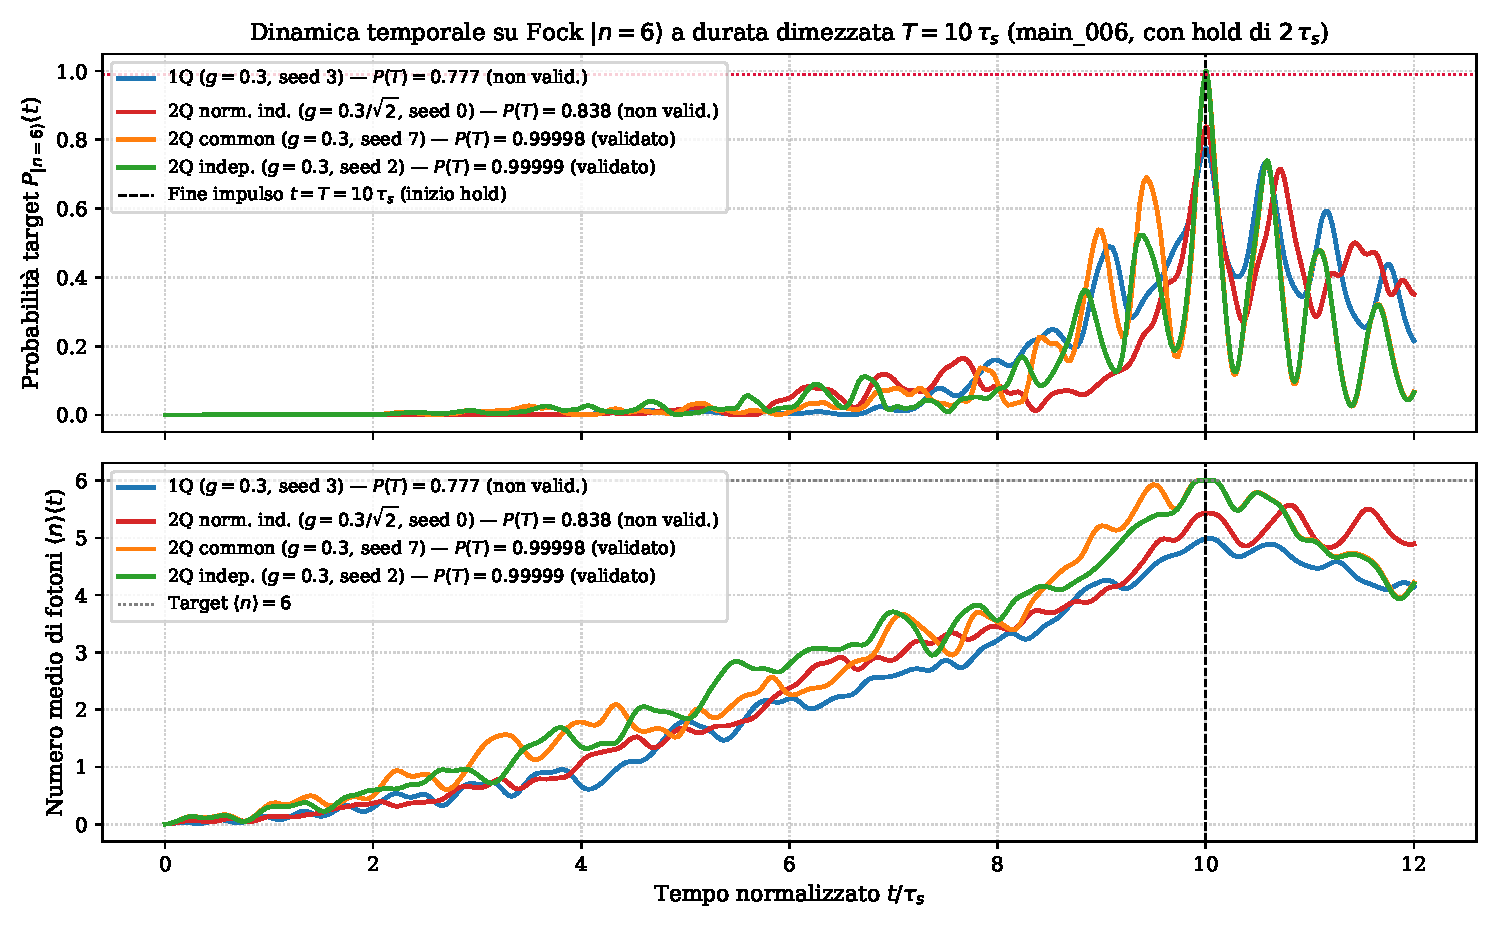
\includegraphics[width=0.96\textwidth]{figure/fig4_dinamica_fock6_t10.pdf}
    \caption{Dinamica temporale della probabilità target $P_{|n=6\rangle}(t)$ (in alto) e del numero medio di fotoni $\langle n \rangle(t)$ (in basso) per Fock $|n=6\rangle$ a durata dimezzata $T = 10\,\tau_s$ (\texttt{main\_006}). Mentre \texttt{1q} e \texttt{2q\_normalized\_independent} non riescono a pompare in media i 6 fotoni entro $10\,\tau_s$, sia \texttt{2q\_common} sia \texttt{2q\_independent} raggiungono $P > 0.99998$ a $t=T$. Dopo $t=10\,\tau_s$ (linea tratteggiata verticale) è visibile la fase di \texttt{hold\_time} a comando spento, in cui lo stato scambia energia con i qubit a causa dell'accoppiamento $g$ sempre attivo.}
    \label{fig:dinamica_fock6_t10}
\end{figure}

\begin{figure}[H]
    \centering
    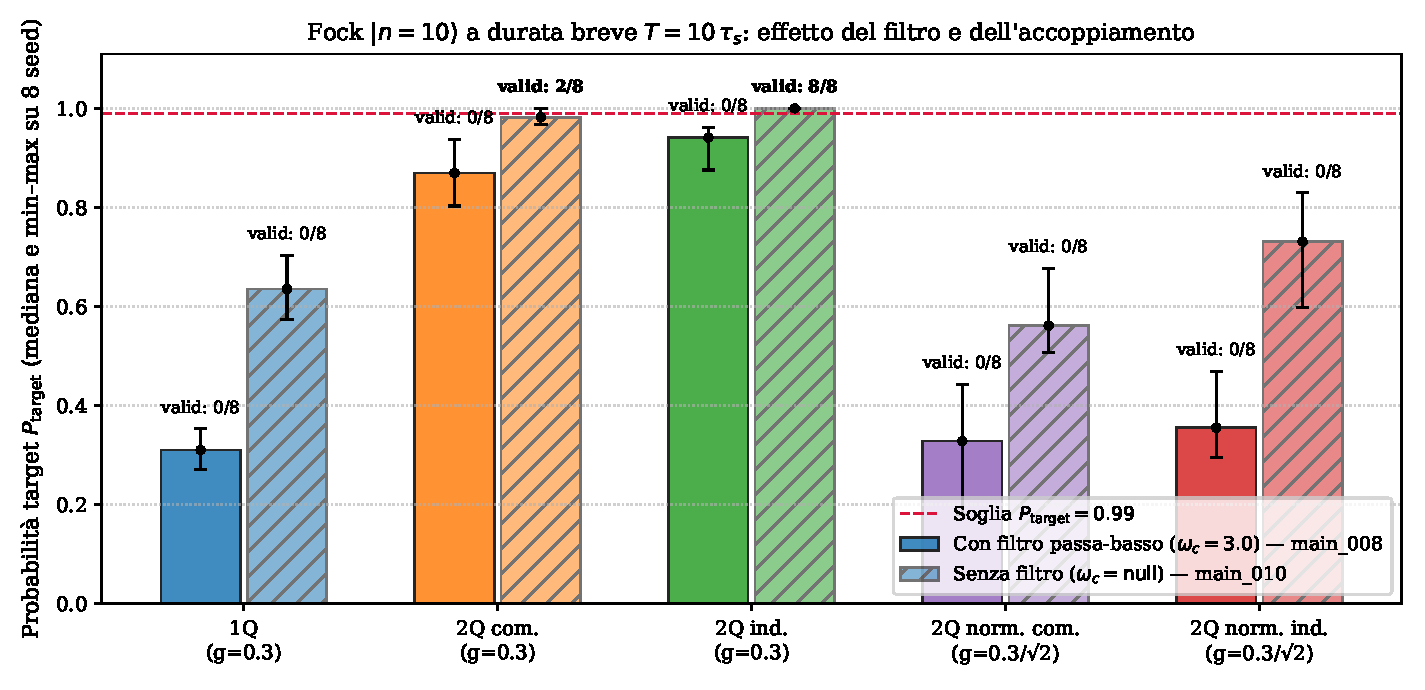
\includegraphics[width=0.92\textwidth]{figure/fig2_fock10_t10_filtro_vs_nofiltro.pdf}
    \caption{Confronto su Fock $|n=10\rangle$ a $T = 10\,\tau_s$ tra il blocco con filtro causale $\omega_{\text{cut}}=3.0$ (\texttt{main\_008}, barre piene) e il blocco diagnostico senza filtro (\texttt{main\_010}, barre tratteggiate). Togliendo il filtro, \texttt{2q\_independent} passa da 0/8 a 8/8 seed validati sopra soglia ($P_{\text{mediana}} = 0.999937$), mentre \texttt{1q} e i casi \texttt{2q\_normalized} restano sotto $0.83$ anche senza filtro.}
    \label{fig:filtro_vs_nofiltro}
\end{figure}

\begin{figure}[H]
    \centering
    \begin{subfigure}[b]{0.48\textwidth}
        \centering
        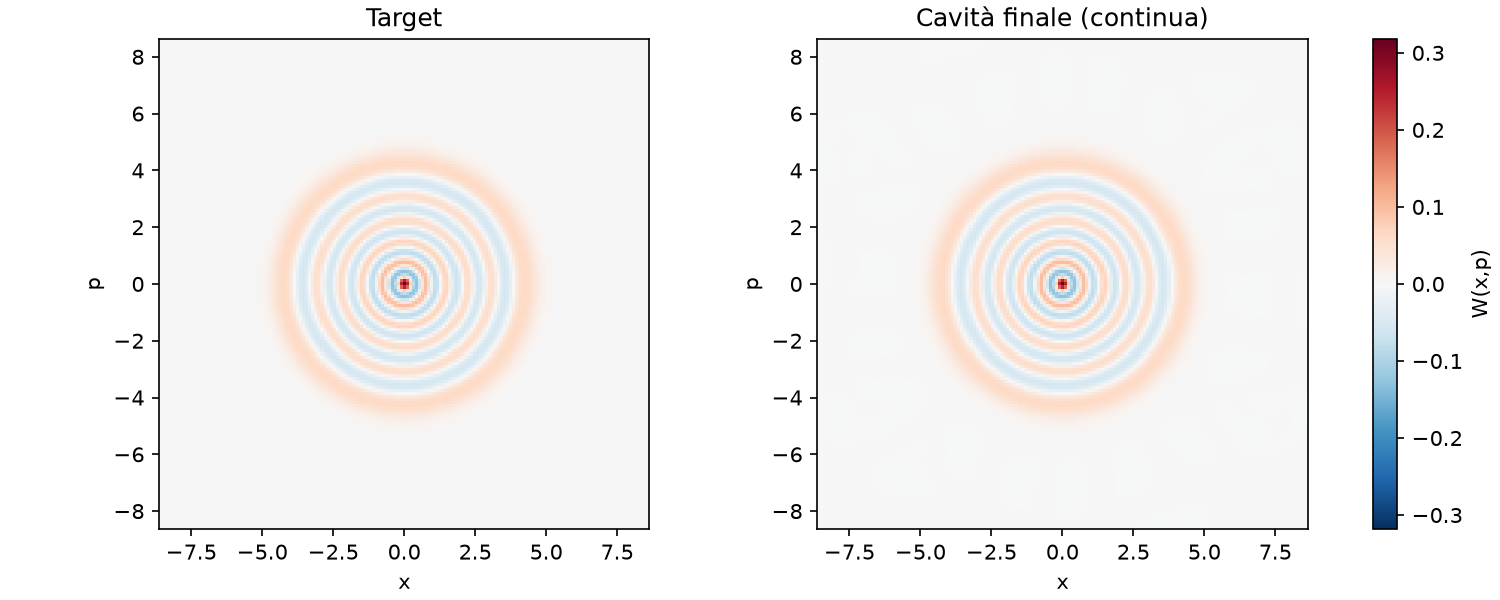
\includegraphics[width=\textwidth]{figure/main009_1q_seed3_wigner.png}
        \caption{\texttt{1q} (seed 3, $T=20\,\tau_s$): $P_{\text{target}} = 0.999995$}
    \end{subfigure}
    \hfill
    \begin{subfigure}[b]{0.48\textwidth}
        \centering
        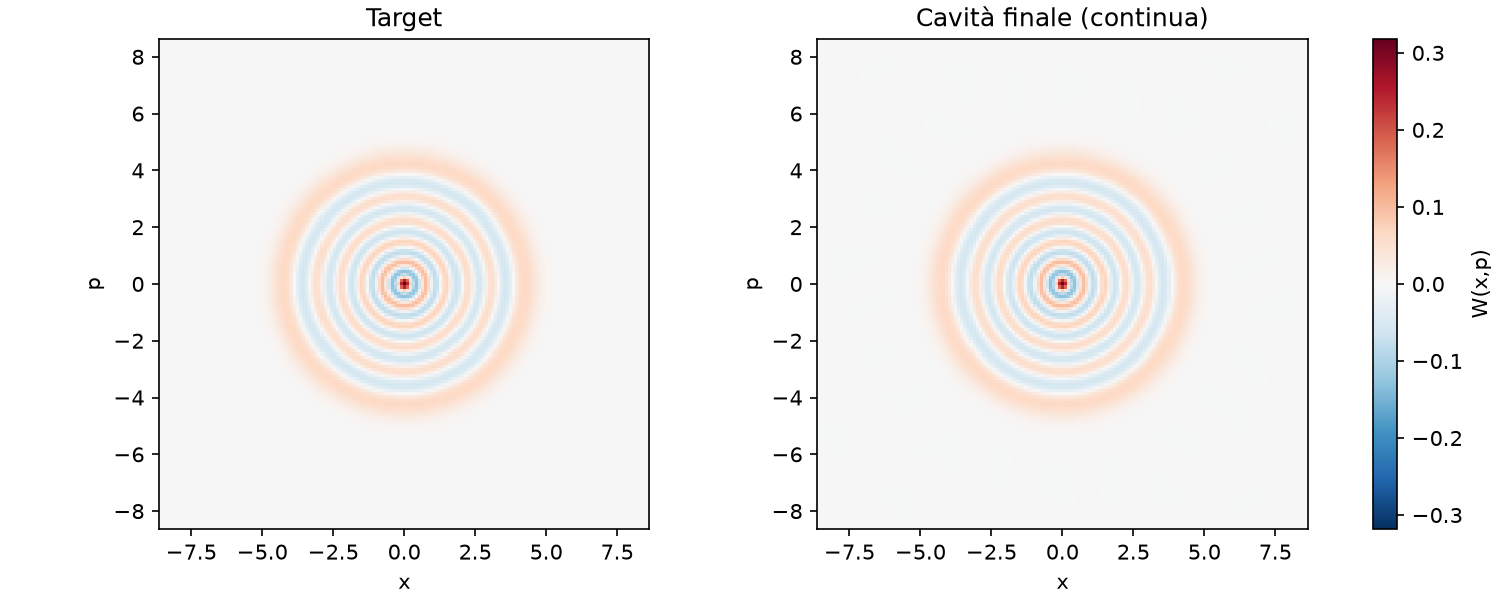
\includegraphics[width=\textwidth]{figure/main009_2q_ind_seed4_wigner.png}
        \caption{\texttt{2q\_independent} (seed 4, $T=20\,\tau_s$): $P_{\text{target}} = 0.999995$}
    \end{subfigure}
    \caption{Funzioni di Wigner (target vs stato finale preparato) per Fock $|n=10\rangle$ a $T=20\,\tau_s$ con filtro $\omega_{\text{cut}}=3.0$ (\texttt{main\_009}): usando l'obiettivo \texttt{root} e portando lo spazio a $\text{dim}=60$, sia il singolo qubit sia i due qubit riproducono i 10 anelli concentrici con precisione certificata.}
    \label{fig:wigner_main009}
\end{figure}

\section{Confronto diretto tra risultati v1 e v2}

Per confrontare i numeri ottenuti prima e dopo il passaggio alla v2, nella Tabella~\ref{tab:confronto_v1_v2} (e in Figura~\ref{fig:confronto_v1_v2}) ho affiancato i casi di Fock che avevo già simulato nella v1. Nel leggere la tabella bisogna tenere conto che:
\begin{itemize}
    \item in \textbf{v1} il valore riportato nei report era la fedeltà radice $F_{\text{root}} = \sqrt{P_{\text{target}}}$ del solo miglior seed CRAB raffinato con GRAPE e poi interpolato con PCHIP (senza filtro nell'ottimizzazione e con $\text{dim}=40$); per un confronto omogeneo ho calcolato anche il quadrato $P_{\text{target}} \approx F_{\text{root}}^2$;
    \item in \textbf{v2} il valore proviene dalla propagazione continua \texttt{sesolve} con filtro causale $\omega_{\text{cut}}=3.0$ incluso nell'ottimizzazione (più il caso senza filtro per $n=10, T=10\,\tau_s$), su 8 seed tutti raffinati e validati a $\text{dim}=60$ vs $80$.
\end{itemize}

\begin{figure}[H]
    \centering
    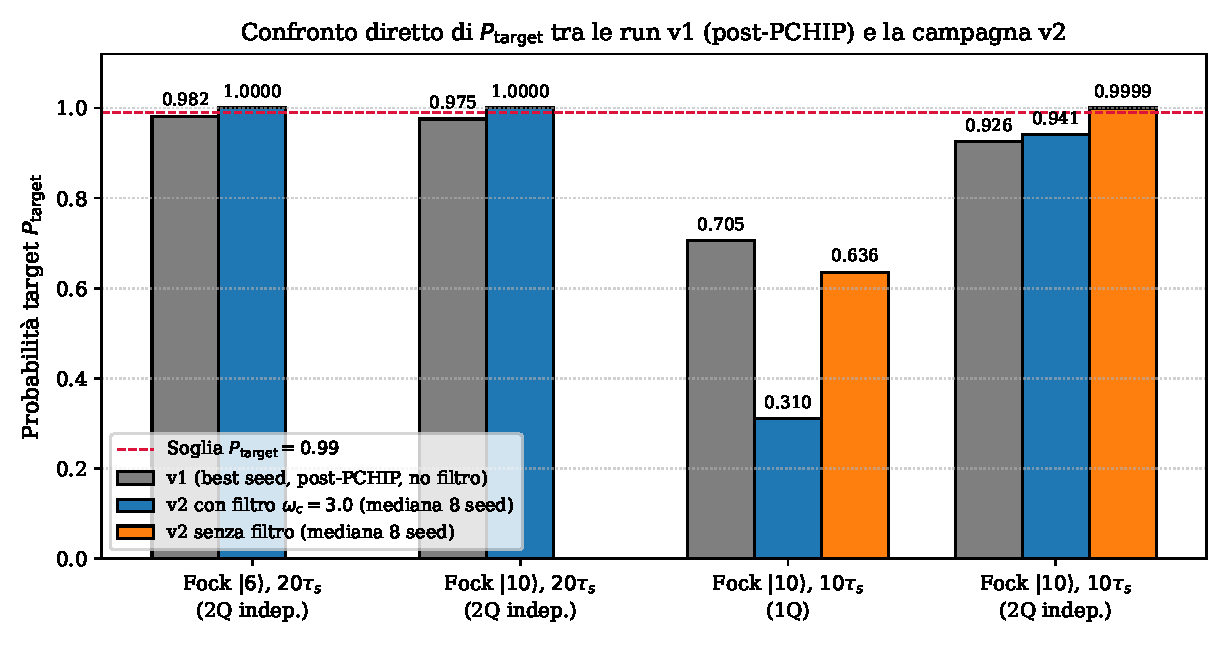
\includegraphics[width=0.78\textwidth]{figure/fig3_confronto_v1_v2.pdf}
    \caption{Confronto diretto della probabilità target $P_{\text{target}}$ tra le run della v1 (dopo smoothing PCHIP) e le mediane della campagna v2 (con e senza filtro).}
    \label{fig:confronto_v1_v2}
\end{figure}

\begin{table}[H]
\centering
\footnotesize
\setlength{\tabcolsep}{4pt}
\renewcommand{\arraystretch}{1.2}
\resizebox{\textwidth}{!}{%
\begin{tabular}{llccc}
\toprule
\textbf{Caso fisico} & \textbf{Metrica} & \textbf{v1 (1 seed, post-PCHIP)} & \textbf{v2 con filtro $3.0$ (8 seed)} & \textbf{v2 senza filtro (8 seed)} \\
\midrule
\multirow{2}{*}{\textbf{Fock $n=6$, $T=20\,\tau_s$ — 2Q ind.}}
 & $F_{\text{root}}$ (best / med.) & $0.990824$ (GRAPE $0.999967$) & $0.999999$ (med. $0.999998$) & — \\
 & $P_{\text{target}}$ (best / med.) & $\approx 0.9817$ & $0.999998$ (med. $0.999996$, \textbf{8/8}) & — \\
\midrule
\multirow{2}{*}{\textbf{Fock $n=10$, $T=20\,\tau_s$ — 2Q ind.}}
 & $F_{\text{root}}$ (best / med.) & $0.987673$ (GRAPE $0.999906$) & $0.999998$ (med. $0.999997$) & \emph{[In corso: \texttt{main\_011}]} \\
 & $P_{\text{target}}$ (best / med.) & $\approx 0.9755$ & $0.999995$ (med. $0.999994$, \textbf{8/8}) & \emph{[In corso: \texttt{main\_011}]} \\
\midrule
\multirow{2}{*}{\textbf{Fock $n=10$, $T=10\,\tau_s$ — 1Q}}
 & $F_{\text{root}}$ (best / med.) & $0.839708$ (GRAPE $0.872035$) & $0.593975$ (med. $0.5569$) & $0.838545$ (med. $0.7972$) \\
 & $P_{\text{target}}$ (best / med.) & $\approx 0.7051$ & $0.352806$ (med. $0.3102$, \textbf{0/8}) & $0.703158$ (med. $0.6355$, \textbf{0/8}) \\
\midrule
\multirow{2}{*}{\textbf{Fock $n=10$, $T=10\,\tau_s$ — 2Q ind.}}
 & $F_{\text{root}}$ (best / med.) & $0.962247$ (GRAPE $0.998764$) & $0.980704$ (med. $0.9700$) & $0.999985$ (med. $0.999968$) \\
 & $P_{\text{target}}$ (best / med.) & $\approx 0.9259$ & $0.961781$ (med. $0.9410$, \textbf{0/8}) & $0.999970$ (med. $0.999937$, \textbf{8/8}) \\
\bottomrule
\end{tabular}%
}
\caption{Confronto diretto tra i risultati della pipeline preliminare v1 e quelli della campagna v2.}
\label{tab:confronto_v1_v2}
\end{table}

\paragraph{Cosa è migliorato, cosa è peggiorato e cosa è rimasto uguale:}
\begin{itemize}
    \item \textbf{Eliminazione della perdita post-smoothing:} in v1, anche quando GRAPE arrivava a $0.9999$, il passaggio a una curva continua con PCHIP faceva scendere $P_{\text{target}}$ a $\approx 0.975 - 0.982$ (a $T=20\,\tau_s$) e a $\approx 0.926$ (a $T=10\,\tau_s$). In v2, ottimizzando direttamente il comando continuo con gradiente esatto, la probabilità continua effettiva resta sopra $0.99999$ a $T=20\,\tau_s$ (anche col filtro attivo) e sopra $0.9999$ a $T=10\,\tau_s$ senza filtro.
    \item \textbf{Coerenza sul caso 1Q a $T=10\,\tau_s$ ($n=10$):} nel caso senza filtro (\texttt{main\_010}) il miglior seed 1Q della v2 ottiene $F_{\text{root}} = 0.8385$ ($P = 0.7032$), cioè praticamente lo stesso valore finale che usciva in v1 dopo PCHIP ($F_{\text{root}} = 0.8397$, $P \approx 0.7051$). La differenza è che in v1 quel risultato nasceva da un passo GRAPE difettoso che aveva peggiorato CRAB, mentre in v2 so che l'ottimizzatore è migliorato rispetto a CRAB ma che l'impulso trovato non supera il controllo \texttt{time\_grid} (sfrutta oscillazioni troppo rapide rispetto al passo di discretizzazione). Con il filtro attivo a $\omega_{\text{cut}}=3.0$ (\texttt{main\_008}), la prestazione di 1Q a $10\,\tau_s$ scende ulteriormente ($P_{\text{mediana}} = 0.310$), perché il filtro impedisce quelle oscillazioni ad alta frequenza.
    \item \textbf{Interpretazione fisica più chiara:} il risultato qualitativo che avevo intravisto in v1 su Fock 10 a $T=10\,\tau_s$ (1Q non ce la fa, 2Q sì) è confermato anche in v2, ma ora posso distinguere il perché: grazie ai casi \texttt{2q\_normalized} introdotti in v2, vedo che il salto di prestazioni a $T=10\,\tau_s$ non dipende semplicemente dall'avere due qubit, ma dal fatto che con $g_1=g_2=0.3$ l'accoppiamento complessivo è $\sqrt{2}$ volte più grande, coadiuvato dalla maggiore libertà dei due canali indipendenti.
\end{itemize}

\section{Aspetti ancora aperti e cosa valuterò dopo l'ultimo main}

\begin{enumerate}
    \item \textbf{Completamento di \texttt{main\_011} (Fock $n=10$, $T=20\,\tau_s$, senza filtro):}
    \todo{inserire qui i risultati di \texttt{main\_011} e verificare se anche \texttt{2q\_normalized\_common} raggiunge 8/8 senza filtro, oltre a confrontare fluenza e banda rispetto a \texttt{main\_009}.}
    \item \textbf{Fallimento del check \texttt{time\_grid} nei tentativi che non raggiungono il target a $T=10\,\tau_s$:}
    In tutti i casi a $T=10\,\tau_s$ dove l'ottimizzatore resta lontano da $P=0.99$ (\texttt{1q} e \texttt{2q\_normalized} in \texttt{main\_006}, \texttt{main\_008}, \texttt{main\_010}, e \texttt{2q} filtrati in \texttt{main\_008}), il controllo \texttt{time\_grid} fallisce perché la differenza di fedeltà tra il propagatore midpoint a $N=1000$ intervalli e l'evoluzione continua \texttt{sesolve} supera la soglia di $10^{-4}$. Quando non riesce a salire di probabilità con una dinamica regolare, GRAPE spinge i nodi a variare rapidamente tra uno step e l'altro per spremere qualche punto percentuale nel propagatore discreto. Per quei casi i numeri continui ($P_{\text{target}}$ da \texttt{sesolve}) indicano chiaramente che il target non viene raggiunto, ma se volessi certificare fino alla quarta cifra decimale il valore massimo ottenibile a $T=10\,\tau_s$ con filtro per \texttt{2q\_independent} ($P \approx 0.96$), dovrei testare quel singolo caso raddoppiando gli intervalli ($N=2000$).
    \item \textbf{Tenuta dello stato dopo $T$ (\texttt{hold\_time}):}
    Nelle simulazioni v2 osservo il sistema per ulteriori $2\,\tau_s$ dopo $T$ a comando spento (come mostrato nella parte destra della Figura~\ref{fig:dinamica_fock6_t10}). Poiché in regime USC l'accoppiamento $g$ con i qubit non viene spento a $t=T$ (e con il filtro attivo c'è anche la coda esponenziale del filtro che si scarica), lo stato di Fock preparato a $t=T$ scambia rapidamente energia con i qubit e la probabilità $P_{\text{target}}$ scende già durante l'hold (arrivando a minimi di $\sim 0.02 - 0.28$ per $n=6$ e $n=10$). Questo è un aspetto fisico del modello con $g$ fisso di cui tener conto.
    \item \textbf{Target Cat e Squeezed in v2:}
    I blocchi per lo stato Cat ($\alpha = 2.0$) e lo stato Squeezed ($3\text{ dB}$) sono già predisposti in \texttt{configurazione\_campagna.jsonc} ma sono stati tenuti disattivati per completare prima lo studio sistematico sugli stati di Fock. Visto quanto lo stato Cat soffriva lo smoothing PCHIP in v1 ($0.999 \to 0.899$), sarà molto interessante vedere quanto guadagna nella v2 con il filtro incluso nell'ottimizzazione.
\end{enumerate}

\end{document}
